\documentclass[11pt]{article}

% macros.tex — Vegas paper notation

% ── Packages ──────────────────────────────────────────────────────────
\usepackage{amsmath,amssymb,amsthm}
\usepackage{stmaryrd}       % \llbracket, \rrbracket
\usepackage{mathtools}       % \coloneqq
\usepackage{xcolor}
\usepackage{hyperref}
\usepackage{cleveref}
\usepackage{booktabs}
\usepackage{enumitem}
\usepackage{mathpartir}      % pretty inference rules (operational semantics)
\usepackage{simplebnf}       % pretty BNF grammars

% ── Theorem environments ──────────────────────────────────────────────
\newtheorem{theorem}{Theorem}[section]
\newtheorem{lemma}[theorem]{Lemma}
\newtheorem{proposition}[theorem]{Proposition}
\newtheorem{corollary}[theorem]{Corollary}
\theoremstyle{definition}
\newtheorem{definition}[theorem]{Definition}
\newtheorem{example}[theorem]{Example}
\theoremstyle{remark}
\newtheorem{remark}[theorem]{Remark}
\newtheorem{notation}[theorem]{Notation}

% ── Players and sets ──────────────────────────────────────────────────
\newcommand{\Players}{\mathcal{I}}

% ── Types and values ──────────────────────────────────────────────────
\newcommand{\Ty}{\mathsf{Ty}}
\newcommand{\Val}{\mathsf{Val}}

% ── Visibility annotations ────────────────────────────────────────────
\newcommand{\pub}{\ensuremath{\mathsf{public}}}
\newcommand{\sealed}{\ensuremath{\mathsf{sealed}}}

% ── Contexts ──────────────────────────────────────────────────────────
\newcommand{\view}[1]{\Gamma\!\!\downarrow_{#1}}       % viewVCtx
\newcommand{\erasectx}[1]{\| #1 \|}                    % eraseVCtx
\newcommand{\erasepub}[1]{\| #1 \|^{\pub}}             % erasePubVCtx (public-only erasure operator)

% ── Constructs ────────────────────────────────────────────────────────
\newcommand{\Ret}{\ensuremath{\mathbf{ret}}}
\newcommand{\Let}{\ensuremath{\mathbf{let}}}
\newcommand{\Sample}{\ensuremath{\mathbf{sample}}}
\newcommand{\Commit}{\ensuremath{\mathbf{commit}}}
\newcommand{\Reveal}{\ensuremath{\mathbf{reveal}}}
\newcommand{\Where}{\ensuremath{\mathbf{where}}}

% ── Small-step operational semantics ──────────────────────────────────
\newcommand{\sconf}[3]{\langle #1 \mathrel{;} #2 \mathrel{;} #3 \rangle} % configuration
\newcommand{\sstep}{\longrightarrow}                  % step relation
\newcommand{\lstep}[1]{\xrightarrow{\,#1\,}}          % labelled step
\newcommand{\sem}[1]{\llbracket #1 \rrbracket}        % evaluation in L
\newcommand{\supp}{\mathop{\mathrm{supp}}}            % support of a weighting
\newcommand{\outcomeof}{\mathsf{outcome}}             % terminal outcome reader

% ── Distributions ─────────────────────────────────────────────────────
\newcommand{\FWeight}[1]{\mathcal{W}(#1)}
\newcommand{\PMF}[1]{\mathrm{PMF}(#1)}

% ── Outcomes ──────────────────────────────────────────────────────────
\newcommand{\Outcome}{\mathcal{O}}

% ── Profiles and strategies ───────────────────────────────────────────
\newcommand{\Profile}{\sigma}

% ── Strategic bridge ──────────────────────────────────────────────────
\newcommand{\KG}{\ensuremath{\mathcal{G}}}
\newcommand{\EU}{\ensuremath{\mathrm{EU}}}

% ── Environments ──────────────────────────────────────────────────────
\newcommand{\Env}{\ensuremath{\mathrm{Env}}}

% ── Misc math ─────────────────────────────────────────────────────────
\newcommand{\NNQ}{\ensuremath{\mathbb{Q}_{\ge 0}}}
\newcommand{\bind}{\mathbin{\gg\!=}}

% ── Lean references ───────────────────────────────────────────────────
\newcommand{\TT}[1]{\texttt{#1}}

% ── Event graphs and configurations ───────────────────────────────────
\newcommand{\EG}{\mathcal{E}}                       % an event graph
\newcommand{\prereq}{\mathrm{prereq}}
\newcommand{\Cfg}{\mathsf{Cfg}}                     % configurations of an EG
\newcommand{\readsOf}{\mathrm{reads}}

% ── Machines ──────────────────────────────────────────────────────────
\newcommand{\State}{\mathsf{S}}
\newcommand{\Action}{\mathsf{A}}

% ── Solution concepts / kernels ───────────────────────────────────────
\newcommand{\Kbeh}{K^{\mathrm{beh}}}
\newcommand{\Kpure}{K^{\mathrm{pure}}}
\newcommand{\Kmix}{K^{\mathrm{mix}}}

% ── Faithfulness-relation shapes (the "forest" vocabulary) ────────────
% Symbols used in the guarantees map: an equivalence, a (one-directional)
% adequacy, and a refinement order.
\newcommand{\eqrel}{\cong}            % equivalence (symmetric)
\newcommand{\adeq}{\vDash}            % adequacy: right object IS the denotation
\newcommand{\ordrel}{\sqsubseteq}     % refinement order

% ── Non-intrusive "status / not-yet-mechanized" note ──────────────────
% A footnote that flags an aspirational or partial item without breaking
% the surrounding narrative.  Used sparingly.
\newcommand{\statusnote}[1]{\footnote{\textit{Status.}~#1}}

% ── Boxes for design notes / Lean correspondence ──────────────────────
\newcommand{\leancorr}[1]{%
  \par\smallskip
  {\raggedright\hbadness=10000\emergencystretch=3em
   \noindent\emph{Lean correspondence.} #1\par}%
  \smallskip}

% ── Lean signature boxes ──────────────────────────────────────────────
% A light-shaded, thin-ruled block for displaying Lean signatures.
% Contents are typeset (not verbatim) so we can mix \TT, math, and Greek
% as the rest of the document already does.
\usepackage[most]{tcolorbox}
\tcbset{
  leanstyle/.style={
    colback=black!3, colframe=black!30, boxrule=0.3pt, arc=1pt,
    left=8pt, right=8pt, top=4pt, bottom=4pt,
    breakable, enhanced jigsaw,
    before skip=4pt, after skip=4pt,
    fontupper=\footnotesize\ttfamily,
  },
}
\newtcolorbox{leanbox}[1][]{leanstyle, #1}


\usepackage[margin=1in]{geometry}
\usepackage{tikz}
\usetikzlibrary{arrows.meta,positioning,fit,calc,shapes.geometric,decorations.pathreplacing}

% Be more tolerant about line breaking, since identifier-heavy paragraphs
% can produce unbreakable tokens longer than a column.
\sloppy
\emergencystretch=3em
\hbadness=10000
\hfuzz=4pt

% Local additions for the supplement.
\renewcommand{\TT}[1]{\texttt{\detokenize{#1}}}
\newcommand{\TODO}[1]{\textcolor{red}{\textbf{TODO:} #1}}
\newcommand{\DefRef}[1]{\hyperref[def:#1]{\TT{#1}}}

\title{VegasCore: A Definitional Supplement\\
\large{A Cross-Discipline Reading Guide for the Lean Mechanization}}
\author{}
\date{}

\begin{document}
\maketitle

\begin{abstract}
This document is a companion to the technical report \emph{VegasCore:
Event-Graph-Native Protocol Semantics}. The report describes the architecture in
the language of types and theorems; this supplement collects the
\emph{definitions with mathematical content} that a careful reader needs in
order to navigate the Lean codebase. Each entry pairs the Lean form with an
ordinary mathematical equivalent and a short prose explanation of what the
construct is for.

The intended audience is twofold. We assume programming-languages background
(typed contexts, monads, dependent types, well-formedness judgements) and
provide informal definitions of the game-theoretic vocabulary; conversely we
assume a reader familiar with Nash equilibria, behavioral strategies, and
finite extensive-form games but new to the Lean formalisation, and explain the
PL machinery in terms they can map to standard game forms.

The supplement is organised bottom-up along the same path as the main report:
the ambient probabilistic and language layers, then visibility-aware syntax,
then well-formedness, then the event graph and its machine semantics,
then native round views, FOSG presentations, kernel games, and the public solution-concept API. It
finishes with a tour of the worked examples.
\end{abstract}

\tableofcontents

% =====================================================================
\section{How To Read This Document}

\subsection{Conventions}
For each definition we present three items: (i) the Lean signature, often
shortened to the names and types that carry mathematical content, with
implementation noise stripped; (ii) a mathematical equivalent in standard
notation; (iii) a short prose paragraph explaining the construct and
\emph{why it exists}. The Lean name is given in monospace
(e.g.~\TT{Vegas.WFProgram}\label{def:Vegas.WFProgram}). Cross-references match the names used in the
main report.

We use the macros from the main paper: $\WFP$, $\Outcome$, $\FWeight{\cdot}$,
$\PMF{\cdot}$, $\bind$, $\Players$, $\view{\cdot}$, $\pubctx{\cdot}$,
$\erasectx{\cdot}$, $\erasepub{\cdot}$, $\Reach$, $\CanReach$. Where the
supplement introduces additional notation we mark it locally.

\subsection{Bird's-eye view}
\label{sec:birdseye}
A Vegas program is a syntactic description of a finite game. Its meaning is
obtained through the layers below, each of which contributes its own
vocabulary. We list them in the order definitions will appear.

\begin{center}
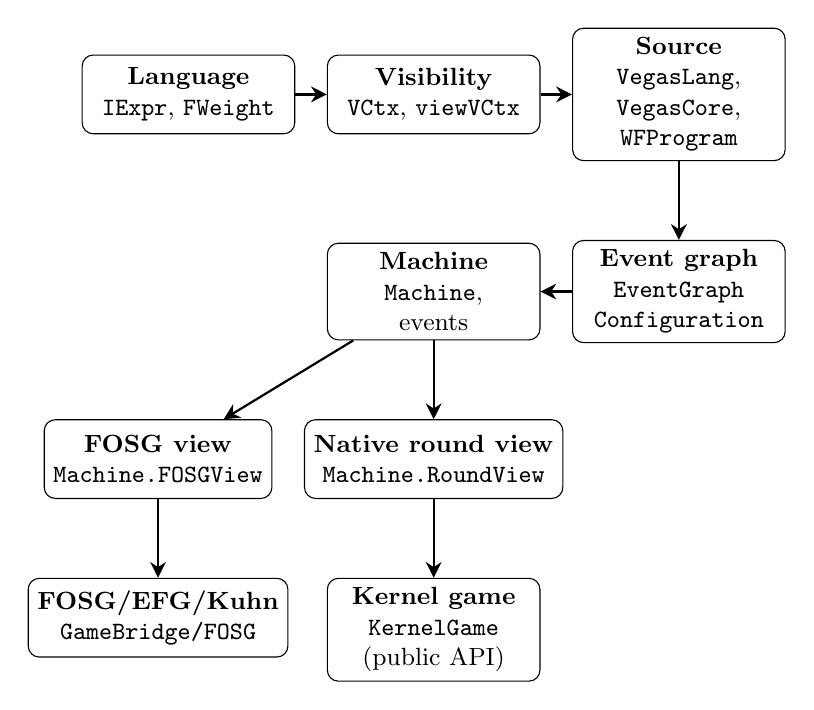
\begin{tikzpicture}[
  every node/.style = {draw, rounded corners, align=center, font=\small,
    minimum width=2.7cm, minimum height=1cm},
  arr/.style = {-{Stealth[length=2mm,width=2mm]}, thick},
]
\node (lang)  {\textbf{Language}\\\TT{IExpr}, \TT{FWeight}};
\node[right=4mm of lang] (vis) {\textbf{Visibility}\\\TT{VCtx}, \TT{viewVCtx}};
\node[right=4mm of vis] (syn) {\textbf{Source}\\\TT{VegasLang},\\\TT{VegasCore},\\\TT{WFProgram}};
\node[below=10mm of syn] (graph) {\textbf{Event graph}\\\TT{EventGraph}\\\TT{Configuration}};
\node[left=4mm of graph] (mach) {\textbf{Machine}\\\TT{Machine},\\events};
\node[below=10mm of mach] (round) {\textbf{Native round view}\\\TT{Machine.RoundView}};
\node[below=10mm of round] (kg) {\textbf{Kernel game}\\\TT{KernelGame}\\(public API)};
\node[left=4mm of round] (fosg) {\textbf{FOSG view}\\\TT{Machine.FOSGView}};
\node[below=10mm of fosg] (efg) {\textbf{FOSG/EFG/Kuhn}\\\TT{GameBridge/FOSG}};
\draw[arr] (lang) -- (vis);
\draw[arr] (vis) -- (syn);
\draw[arr] (syn) -- (graph);
\draw[arr] (graph) -- (mach);
\draw[arr] (mach) -- (round);
\draw[arr] (round) -- (kg);
\draw[arr] (mach) -- (fosg);
\draw[arr] (fosg) -- (efg);
\end{tikzpicture}
\end{center}

\noindent The arrows are read as ``defines on top of''. The substantive
mathematical work happens at the event-graph level, where a syntax tree
is turned into a DAG with \emph{extensional} state — the configuration
records only which nodes have produced which results, not the schedule
that produced them — and at the native round-view level, where the
game-theoretic strategy carriers are recovered.  The FOSG branch is a
presentation/proof bridge used for EFG and Kuhn theorems.

\subsection{Code organisation}
\label{sec:code-organisation}\label{def:Lang.ToCore}\label{def:Core.ToEventGraph}\label{def:EventGraph.ToMachine}\label{def:Fields}\label{def:Obligations}\label{def:Construction}

The Lean modules follow the semantic ownership of the construction, not a
single compiler package.  The internal Vegas pipeline uses source-owned
\TT{ToX}\label{def:ToX} names:
\[
  \TT{Lang.ToCore}
  \;\longrightarrow\;
  \TT{Core.ToEventGraph}
  \;\longrightarrow\;
  \TT{EventGraph.ToMachine}.
\]
These are the definitional arrows of Vegas itself.  In contrast,
\TT{GameBridge/} contains presentation bridges from the Vegas machine
semantics to FOSG and EFG infrastructure.  Operational implementation
refinement lives in \TT{Backend/}; it is not a game-form bridge.  The
current Vegas-facing strategic carriers in \TT{Strategic/} are built from
the bounded native round view of the event-graph machine.  The bounded FOSG
view is now a presentation bridge used by FOSG/EFG/Kuhn results, not the
definition of the native strategy layer.

\begin{center}\small
\begin{tabular}{@{}p{0.25\textwidth}p{0.66\textwidth}@{}}
\toprule
Folder & Role \\
\midrule
\TT{Base/}
  & Common finite-weight, expression, context, visibility, environment, and
    payoff infrastructure shared by core syntax and event graphs. \\
\TT{Lang/}
  & Concrete/surface language layers, including \TT{VegasLang} and its
    lowering to \TT{VegasCore}. \\
\TT{Core/}
  & \TT{VegasCore}, static well-formedness, checked programs, view kernels,
    and the elaboration \TT{Core.ToEventGraph}.  The elaboration is split into
    \TT{ToEventGraph/Nodes}, \TT{Fields}, \TT{Obligations}, and
    \TT{Construction}. \\
\TT{EventGraph/}
  & The central event-graph object, configurations, frontier facts, and the
    internal interpretation \TT{EventGraph.ToMachine}. \\
\TT{Machine/}
  & Generic operational machine carrier, native round views, and primitive
    trace semantics. \\
\TT{Strategic/}
  & Vegas-facing strategic API: native strategy carriers, game forms,
    kernel games, expected utility, equilibrium vocabulary, dominance, and
    transport. \\
\TT{GameBridge/}
  & Bridges from Vegas semantics to FOSG/EFG machinery and the FOSG Kuhn
    realisation theorem, including native/FOSG equivalence theorems that
    transport those results back to the native API. \\
\TT{Backend/}
  & Runtime/backend refinement obligations and backend blocked-trace
    kernel-game transport. \\
\TT{Export/}
  & Thin export-facing API for finite pure kernel games; currently an oracle
    and enumeration package, not a solver file writer. \\
\bottomrule
\end{tabular}
\end{center}

\subsection{A glossary for the cross-disciplinary reader}

\paragraph{For PL readers.}
A \emph{(finite) game} consists of a player set $\Players$, per-player action
sets, and a probabilistic mechanism that turns chosen profiles into payoff
vectors. A \emph{strategy} is what a player intends to do; a \emph{profile} is
one strategy per player. \emph{Expected utility} $\EU$ is the expected payoff
under a profile. \emph{Nash equilibrium} is a profile from which no player
gains by unilateral deviation. \emph{Mixed} strategies randomise over pure
ones; \emph{behavioral} strategies randomise locally at each information set.
\emph{Kuhn's theorem} says that under perfect recall mixed and behavioral
strategies are equivalent. A \emph{factored-observation stochastic game} (FOSG)
is the modern formalism for finite extensive-form games with imperfect
information; players observe local signals at each round.

\paragraph{For game-theory readers.}
A \emph{typed context} $\VCtx$ is just a list of $(\text{name}, \text{type})$
pairs, like a typing environment in a static type checker. A
\emph{de~Bruijn-like} membership proof \TT{HasVar}\label{def:HasVar}~$\Gamma$~$x$~$\tau$ is the
evidence that variable $x$ has type $\tau$ in $\Gamma$. A
\emph{well-formedness} predicate is a side condition collected by the type
checker (here: bindings have unique names, every commitment is revealed,
distributions sum to one, every commit can be played by at least one
action). \emph{Erasure} forgets the visibility annotation on a context to
hand the result to a plain expression evaluator. The \emph{denotation
brackets} $\den{p}$ are not needed for individual definitions; they are
bookkeeping for ``the meaning of $p$''.

\paragraph{A two-column glossary.}

\begin{center}\small
\begin{tabular}{@{}p{0.32\textwidth}p{0.6\textwidth}@{}}
\toprule
PL term & Game-theoretic counterpart \\
\midrule
typed binding $(x, \pub\,\tau)$
  & a public observation channel of type $\tau$ \\
typed binding $(x, \hid\,p\,\tau)$
  & a sealed move/private signal of player $p$ \\
\Sample~$x \sim D$
  & a chance node drawn from $D$, observable by all \\
\Commit{} (player $p$) $x \mid R$
  & a player-$p$ move at an information set; $R$ is the legality predicate \\
\Reveal~$y := x$
  & a public announcement of a previously sealed value \\
\Ret~$\bar{p}$
  & terminal node carrying the payoff vector $\bar p$ \\
\midrule
\TT{EventGraph}
  & the game tree, but DAG-shaped and order-quotiented \\
\TT{Configuration}
  & a partially-played history (closed under causal deps) \\
frontier of a configuration
  & set of currently-active moves \\
\TT{Machine}
  & operational carrier of the game \\
\TT{Machine.FOSGView}
  & the same game read at round-level, with information sets \\
\TT{KernelGame}
  & strategic-form game (strategies, outcome kernel, utility) \\
\TT{pureKernelGame}, \TT{pmfBehavioralKernelGame}
  & finite normal-form / behavioral-form view of a Vegas program \\
\bottomrule
\end{tabular}
\end{center}

% =====================================================================
\section{The Probability and Language Layer}

\subsection{Finite-support weights: \TT{FWeight}}
\label{def:FWeight}

\begin{leanbox}
abbrev FWeight ($\alpha$ : Type) [DecidableEq $\alpha$] := $\alpha \to_0 \mathbb{Q}_{\ge 0}$\\[1pt]
def pure       : $\alpha \to$ FWeight $\alpha$\label{def:pure}\\
def zero       : FWeight $\alpha$\label{def:zero}\\
noncomputable def bind : FWeight $\alpha \to (\alpha \to$ FWeight $\beta) \to$ FWeight $\beta$\label{def:bind}\\
noncomputable def map  : $(\alpha \to \beta) \to$ FWeight $\alpha \to$ FWeight $\beta$\label{def:map}\\
def ofList      : List $(\alpha \times \mathbb{Q}_{\ge 0}) \to$ FWeight $\alpha$\label{def:ofList}\\
def totalWeight : FWeight $\alpha \to \mathbb{Q}_{\ge 0}$\label{def:totalWeight}\\
def Normalized (d : FWeight $\alpha$) : Prop := d.totalWeight = 1\\
def toPMF (d : FWeight $\alpha$) : d.Normalized $\to$ PMF $\alpha$\label{def:toPMF}
\end{leanbox}

A value of type $\FWeight{\alpha}$ is a finitely-supported,
non-negative-rational weight function on $\alpha$. Writing $w(\mu)$ for
the total mass and abbreviating Iverson brackets $[P]$,
\begin{align*}
  \FWeight{\alpha} &\;:=\; \bigl\{\, \mu : \alpha \to \NNQ \;\bigm|\; |\mathrm{supp}\,\mu| < \infty \,\bigr\}, \\
  w(\mu) &\;:=\; \textstyle\sum_{a} \mu(a) \;\in\; \NNQ, \\
  \mathrm{pure}(x)(a) &\;:=\; [\,a = x\,], \\
  (\mu \bind f)(b) &\;:=\; \textstyle\sum_{a} \mu(a)\cdot f(a)(b), \\
  (\mathrm{map}\,g\,\mu)(b) &\;:=\; \textstyle\sum_{a : g(a)=b} \mu(a).
\end{align*}
Normalized weights — those with $w(\mu) = 1$ — are written
\TT{FProb}\label{def:FProb} in Lean. The trio $(\mathrm{pure}, \bind, \mathrm{map})$
is the standard structure of a probability monad: $\mathrm{pure}$ injects a
value as a Dirac mass, $\bind$ sequences a stochastic step with a
continuation indexed by its result, and $\mathrm{map}$ is the pushforward
through a deterministic function.

\paragraph{Why this and not $\PMF{\cdot}$.}
(i)~Raw weights let intermediate \TT{bind}-trees be built without
per-step normalisation proofs. (ii)~Rational weights are decidably equal,
so concrete examples are mechanically inspectable. (iii)~Decidable
equality on $\alpha$ is required to construct the underlying \TT{Finsupp}
computably. \TT{toPMF} requires a proof of $w(\mu) = 1$ and is the only
bridge from $\FWeight{\cdot}$ into Mathlib's measure-theoretic $\PMF{\cdot}$.

\paragraph{Key laws.}
The monad laws hold (left/right identity of $\mathrm{pure}$, associativity
of $\bind$). Finite weights \emph{commute},
\[
  \mu_1 \bind \lambda x.\, \mu_2 \bind \lambda y.\, f(x,y)
  \;=\;
  \mu_2 \bind \lambda y.\, \mu_1 \bind \lambda x.\, f(x,y),
\]
which licenses commit-commit commutation in the program semantics.
Normalisation is preserved by $\bind$: if $w(\mu) = 1$ and $w(f(a)) = 1$
for every $a \in \mathrm{supp}(\mu)$, then $w(\mu \bind f) = 1$.

\subsection{The expression-language interface: \TT{IExpr}}
\label{def:IExpr}

\DefRef{IExpr} is the abstract interface a Vegas program needs in order
to type-check its expressions and distributions. It bundles five pieces
of data — a typed universe, two distinguished base types, deterministic
and distribution-valued syntax with their evaluators, and static
dependency analyses — together with five laws tying the data together.
Throughout, $\Gamma$ ranges over \TT{Ctx Ty} and $\tau, \sigma, b$ over
\TT{Ty}; implicit binders for these are suppressed in the boxes below.

\begin{leanbox}
structure IExpr where\\[1pt]
\bd Ty       : Type\\
\bd Val      : Ty $\to$ Type\\
\bd decEqTy  : DecidableEq Ty\\
\bd decEqVal : $\forall$ \{$\tau$\}, DecidableEq (Val $\tau$)\\[2pt]
\bd bool     : Ty\label{def:Bool}\\
\bd toBool   : Val bool $\to$ Bool\\
\bd int      : Ty\label{def:Int}\\
\bd toInt    : Val int  $\to$ Int\\[2pt]
\bd Expr     : Ctx Ty $\to$ Ty $\to$ Type\label{def:Expr}\\
\bd eval     : Expr $\Gamma\,\tau \to$ Env Val $\Gamma \to$ Val $\tau$\label{def:eval}\\[2pt]
\bd DistExpr : Ctx Ty $\to$ Ty $\to$ Type\label{def:DistExpr}\\
\bd evalDist : DistExpr $\Gamma\,\tau \to$ Env Val $\Gamma \to$ FWeight (Val $\tau$)\label{def:evalDist}\\[2pt]
\bd exprDeps : Expr $\Gamma\,\tau \to$ Finset VarId\label{def:exprDeps}\\
\bd distDeps : DistExpr $\Gamma\,\tau \to$ Finset VarId\label{def:distDeps}\\[1pt]
\bd -- laws follow
\end{leanbox}

\noindent The five field groups, separated by blank lines, play distinct roles.

\begin{itemize}\itemsep2pt
\item \emph{Typed universe.}
  $\TT{Ty}$ is a Lean-level universe of embedded-language types;
  $\TT{Val}$ associates to each $\tau \in \TT{Ty}$ the Lean type of its
  values. Decidable equality on $\TT{Ty}$ and on each $\TT{Val}\,\tau$
  is required for $\FW$-backed distributions to type-check
  downstream; both are promoted to typeclass instances at structure
  boundary.
\item \emph{Distinguished base types.}
  Two specific elements of $\TT{Ty}$ are named, with projections into
  Lean's \DefRef{Bool} and \DefRef{Int}. Commit guards return
  $\TT{Val}\,\TT{bool}$ and are read out via $\TT{toBool}$; per-player
  payoffs return $\TT{Val}\,\TT{int}$ and are read out via $\TT{toInt}$.
\item \emph{Expression syntax.}
  $\DefRef{Expr}\,\Gamma\,\tau$ is the Lean type of well-typed
  expressions over $\Gamma$ of type $\tau$.
  $\DefRef{eval}\,e\,\rho$ is its denotation against an environment
  $\rho \in \Env_{\TT{Val}}\Gamma$.
\item \emph{Distribution syntax.} The same shape with
  $\DefRef{DistExpr}\,\Gamma\,\tau$ inhabited by syntactic descriptions
  of finite distributions over $\TT{Val}\,\tau$, and \DefRef{evalDist}
  producing the corresponding $\FWeight{\TT{Val}\,\tau}$.
\item \emph{Static dependency analyses.}
  $\DefRef{exprDeps}\,e$ and $\DefRef{distDeps}\,d$ are syntactically
  computed finite sets of variable identifiers. The intent is that
  they over-approximate the variables an expression reads; the laws
  pin down what ``reads'' means.
\end{itemize}

\begin{leanbox}
\bd -- ...continued\\[1pt]
\bd expr\_deps\_context :\label{def:expr_deps_context}\\
\bdd $\forall$ (e : Expr $\Gamma\,\tau$),\\
\bdd \ \ $\forall$ x, x $\in$ exprDeps e $\to$ x $\in \Gamma$.map Prod.fst\\[3pt]
\bd extendAfterHead :\label{def:extendAfterHead}\\
\bdd $\forall$ (e : Expr ((x,$\tau$)::$\Gamma$) b),\\
\bdd \ \ $\exists$ e' : Expr ((x,$\tau$)::(y,$\sigma$)::$\Gamma$) b,\\
\bdd \ \ \ \ $\forall$ vx vy $\rho$,\\
\bdd \ \ \ \ \ \ eval e' (vx, vy, $\rho$) = eval e (vx, $\rho$)\\[3pt]
\bd dropAfterHead :\label{def:dropAfterHead}\\
\bdd $\forall$ (e : Expr ((x,$\tau$)::(y,$\sigma$)::$\Gamma$) b),\\
\bdd \ \ y $\notin$ exprDeps e $\to$\\
\bdd \ \ $\exists$ e' : Expr ((x,$\tau$)::$\Gamma$) b,\\
\bdd \ \ \ \ $\forall$ vx vy $\rho$,\\
\bdd \ \ \ \ \ \ eval e' (vx, $\rho$) = eval e (vx, vy, $\rho$)\\[3pt]
\bd expr\_deps\_sound :\label{def:expr_deps_sound}\\
\bdd $\forall$ (e : Expr $\Gamma\,\tau$) ($\rho_1\,\rho_2$ : Env Val $\Gamma$),\\
\bdd \ \ AgreesOn $\rho_1\,\rho_2$ (exprDeps e) $\to$\\
\bdd \ \ \ \ eval e $\rho_1$ = eval e $\rho_2$\\[3pt]
\bd dist\_deps\_sound :\label{def:dist_deps_sound}\\
\bdd $\forall$ (d : DistExpr $\Gamma\,\tau$) ($\rho_1\,\rho_2$ : Env Val $\Gamma$),\\
\bdd \ \ AgreesOn $\rho_1\,\rho_2$ (distDeps d) $\to$\\
\bdd \ \ \ \ evalDist d $\rho_1$ = evalDist d $\rho_2$
\end{leanbox}

\noindent The five laws decompose into three groups.

\begin{itemize}\itemsep2pt
\item \emph{Well-typing of the dependency analysis}
  (\DefRef{expr_deps_context}): every variable identifier reported by
  $\mathtt{exprDeps}\,e$ already names a binding in $\Gamma$,
  \[
    \mathtt{exprDeps}\,e \;\subseteq\; \mathrm{names}(\Gamma).
  \]
\item \emph{Structural weakening}
  (\DefRef{extendAfterHead}, \DefRef{dropAfterHead}): an expression in
  context $(x,\tau)::\Gamma$ may be transported to
  $(x,\tau)::(y,\sigma)::\Gamma$ by inserting an unrelated binding
  after the head, and conversely a binding the expression does not
  depend on may be removed. Symbolically, with $\mathtt{eval}\,e\,\rho$
  the denotation,
  \begin{align*}
    \forall e \in \Expr((x,\tau)::\Gamma, b).\;
    \exists\, e'.\;\;
    & \mathtt{eval}\,e'\,(\langle x{=}vx\rangle\langle y{=}vy\rangle\rho)
      = \mathtt{eval}\,e\,(\langle x{=}vx\rangle\rho), \\
    \forall e \in \Expr((x,\tau)::(y,\sigma)::\Gamma, b),\;
    y \notin \mathtt{exprDeps}\,e.\;
    \exists\, e'.\;\;
    & \mathtt{eval}\,e'\,(\langle x{=}vx\rangle\rho)
      = \mathtt{eval}\,e\,(\langle x{=}vx\rangle\langle y{=}vy\rangle\rho).
  \end{align*}
  These two laws license commit-commit commutativity in the program
  semantics: an expression evaluated past one binding can be
  reformulated past two, and back.
\item \emph{Dependency soundness}
  (\DefRef{expr_deps_sound}, \DefRef{dist_deps_sound}): if two
  environments agree on the declared dependencies, evaluation is
  identical:
  \[
    \mathrm{AgreesOn}(\rho_1, \rho_2, \mathtt{exprDeps}\,e) \;\implies\;
    \mathtt{eval}\,e\,\rho_1 = \mathtt{eval}\,e\,\rho_2,
  \]
  and likewise $\mathtt{distDeps} \implies \mathtt{evalDist}$. This is
  the key semantic property: $\mathtt{exprDeps}$ may over-report variable
  reads but it cannot \emph{miss} a read that affects the value.
\end{itemize}

\paragraph{Trusted interface obligation.}
The Vegas proofs never inspect the internal syntax of an expression
language; they consume \DefRef{IExpr} purely through these laws. An
instance may over-report dependencies, but it cannot under-report a
semantically relevant read and still satisfy \DefRef{expr_deps_sound}
or \DefRef{dist_deps_sound}.

\paragraph{Concrete instance.}
\DefRef{simpleExpr}\label{def:simpleExpr} instantiates \DefRef{IExpr}
with
\[
  \Ty = \{\intt,\,\bool,\,\mathsf{range}\,\ell\,h,\,\mathsf{option}\,b\},
  \qquad
  \Val(\mathsf{option}\,b) = \mathrm{Option}(\Val(b)),
\]
and an expression syntax containing constants, addition, equality,
boolean conjunction and negation, $\TT{ite}$, and option
constructors/eliminators
\DefRef{none}\label{def:none},
\DefRef{some}\label{def:some},
\DefRef{isSome}\label{def:isSome},
\DefRef{isNone}\label{def:isNone},
\DefRef{getD}\label{def:getD};
distributions are built either as weighted lists of $(v, q)$ pairs or
by guarded choice. All \TT{VegasLang} programs in this development use
\DefRef{simpleExpr}.

Two type classes accompany the concrete instance and are not part of
the generic \DefRef{IExpr} interface:
\begin{itemize}\itemsep1pt
\item \DefRef{CommitPayloadTy}\label{def:CommitPayloadTy} marks the
  non-nullable types admissible as explicit surface commit payloads.
  The lemma
  \DefRef{not_commitPayloadTy_option}\label{def:not_commitPayloadTy_option}
  rules out explicit user commits at type \TT{BaseTy.option b}.
\item \DefRef{DefaultVal}\label{def:DefaultVal} supplies the fallback
  used to lift a guard over $b$ to a guard over \TT{option b}, fired
  only under \DefRef{getD} in the non-null branch.
\end{itemize}
A different expression language would supply its own option type,
non-nullable predicate, and default-value class to support the
nullable yield layer.

\subsection{Plain typed contexts: \TT{Ctx}, \TT{HasVar}, \TT{Env}}
\label{def:Ctx}

\begin{leanbox}
abbrev VarId : Type := Nat\label{def:VarId}\\
abbrev Ctx (Ty : Type) := List (VarId $\times$ Ty)\\[2pt]
inductive HasVar : Ctx Ty $\to$ VarId $\to$ Ty $\to$ Type\label{def:Type} where\\
\bd | here  : HasVar ((x, $\tau$) :: $\Gamma$) x $\tau$\\
\bd | there : HasVar $\Gamma$ x $\tau$ $\to$ HasVar ((y, $\tau'$) :: $\Gamma$) x $\tau$\\[2pt]
def Env (Val : Ty $\to$ Type)\label{def:Val} : Ctx Ty $\to$ Type :=\\
\bd fun $\Gamma\Rightarrow \forall$ x $\tau$, HasVar $\Gamma$ x $\tau \to$ Val $\tau$
\end{leanbox}

A \emph{context} $\Gamma$ is a list of typed variable bindings, and an
\emph{environment} $\rho \in \Env(\Gamma)$ assigns a value to each.
$\TT{HasVar}\,\Gamma\,x\,\tau$ is a typed de~Bruijn membership witness.
Under $\TT{Nodup}(\Gamma.\TT{map}\,\TT{fst})$\label{def:Nodup} — no
repeated names — \TT{HasVar} is a subsingleton (any two witnesses are
equal), so $\Env$-lookup is proof-irrelevant: the retrieved value depends
on $x$ and $\tau$ only, not on the chosen witness.

\paragraph{Why \TT{HasVar} is in \TT{Type}, not \TT{Prop}.}
$\Env$ pattern-matches on \TT{HasVar} to retrieve values, which requires it
to live in the data universe. The single lemma
\TT{Env.get_eq_of_nodup}\label{def:Env.get_eq_of_nodup}\label{def:Env}
discharges the resulting proof-position equality once and for all.

% =====================================================================
\section{Visibility-aware Syntax}

The protocol layer is concerned not just with variables but with
\emph{who can see which variable}. The standard PL apparatus is extended
with a visibility tag on each binding. Throughout this section, \TT{P}
is the player type with \TT{[DecidableEq P]} and \TT{L} is an
\DefRef{IExpr} instance.

\subsection{Visibility tags: \TT{BindTy}}
\label{def:BindTy}

\begin{leanbox}
inductive Visibility (Player : Type) where\\
\bd | pub\label{def:pub}\\
\bd | hidden (owner : Player)\\[3pt]
structure BindTy (Player : Type) (L : IExpr) where\\
\bd base       : L.Ty\\
\bd visibility : Visibility Player
\end{leanbox}

A binding type is either \emph{public} ($\pub\,\tau$, visible to all) or
\emph{hidden} ($\hid\,p\,\tau$, visible only to its owner $p$). The
information model is \emph{owner-or-all}: a secret either belongs to one
player, or is visible to everyone — there is no group-visibility
constructor. The base type and visibility are independent fields:
reveal-like operations change visibility by introducing a fresh public
alias, not by mutating the variable's base type. Smart constructors
$\TT{BindTy.pub}\,\tau$ and $\TT{BindTy.hidden}\,p\,\tau$ keep call
sites readable while preserving the split representation.

\subsection{Visibility contexts and views: \TT{VCtx}, \TT{viewVCtx}, \TT{pubVCtx}}
\label{def:VCtx}\label{def:pubVCtx}\label{def:viewVCtx}

\begin{leanbox}
abbrev VCtx (P : Type) (L : IExpr) : Type :=\\
\bd List (VarId $\times$ BindTy P L)\\[3pt]
def viewVCtx (p : P) : VCtx P L $\to$ VCtx P L\\
def pubVCtx          : VCtx P L $\to$ VCtx P L
\end{leanbox}

\DefRef{viewVCtx}~$p$ keeps only bindings player $p$ can see — public
bindings and hidden bindings owned by $p$. \DefRef{pubVCtx} keeps only
the public sublist. Writing $\view{p}$ for the player-$p$ view and
$\pubctx{\Gamma}$ for the public fragment,
\[
  \view{p} \;=\;
    \bigl[(x, \tau) \in \Gamma \;\big|\; p \text{ can see } \tau\bigr],
  \qquad
  \pubctx{\Gamma} \;=\;
    \bigl[(x, \pub\,\tau) \in \Gamma\bigr].
\]
Public bindings are visible to every player, so $\pubctx{\Gamma}
\subseteq \view{p}$ pointwise.

\subsection{Erasure to plain contexts: \TT{eraseVCtx}, \TT{erasePubVCtx}}
\label{def:erase}\label{def:erasePubVCtx}\label{def:eraseVCtx}

\begin{leanbox}
def eraseVCtx    : VCtx P L $\to$ Ctx L.Ty\\
def erasePubVCtx : VCtx P L $\to$ Ctx L.Ty
\end{leanbox}

\DefRef{eraseVCtx} forgets visibility tags entirely;
\DefRef{erasePubVCtx} forgets visibility tags after restricting to the
public sublist:
\[
  \erasectx{\Gamma} \;=\;
    [(x, \tau.\mathrm{base}) \mid (x,\tau) \in \Gamma],
  \qquad
  \erasepub{\Gamma} \;=\;
    [(x, \tau) \mid (x, \pub\,\tau) \in \Gamma].
\]
The commutation lemma
\DefRef{eraseVCtx_pubVCtx}\label{def:eraseVCtx_pubVCtx} says these two
projections — public-restrict, then forget; or forget after
public-restrict — produce the same plain context:
\[
  \erasectx{\pubctx{\Gamma}} \;=\; \erasepub{\Gamma}.
\]

\paragraph{Why two erasures.}
The full erased context $\erasectx{\Gamma}$ is what \emph{commit guards}
and operational machinery type over: a guard may syntactically mention
any variable, with a separate predicate restricting what it actually
depends on. The public-only erased context $\erasepub{\Gamma}$ is what
\emph{deterministic let-bindings, samples, and payoff expressions} type
over, since these may not read hidden state. The split is the single
design commitment around which the rest of the development is
organised.

\subsection{Source syntax: \TT{VegasCore}}
\label{def:VegasCore}

\begin{leanbox}
inductive VegasCore (P : Type) [DecidableEq P] (L : IExpr) :\\
\bd VCtx P L $\to$ Type where\\[2pt]
\bd | ret \{$\Gamma$\}\\
\bdd (payoffs : List (P $\times$ L.Expr (erasePubVCtx $\Gamma$) L.int)) :\\
\bdd VegasCore P L $\Gamma$\\[3pt]
\bd | letExpr \{$\Gamma$\} (x : VarId) \{b : L.Ty\}\\
\bdd (e : L.Expr (erasePubVCtx $\Gamma$) b)\\
\bdd (k : VegasCore P L ((x, .pub b) :: $\Gamma$)) :\\
\bdd VegasCore P L $\Gamma$\\[3pt]
\bd | sample \{$\Gamma$\} (x : VarId) \{b : L.Ty\}\\
\bdd (D : L.DistExpr (erasePubVCtx $\Gamma$) b)\\
\bdd (k : VegasCore P L ((x, .pub b) :: $\Gamma$)) :\\
\bdd VegasCore P L $\Gamma$\\[3pt]
\bd | commit \{$\Gamma$\} (x : VarId) (who : P) \{b : L.Ty\}\\
\bdd (R : L.Expr ((x, b) :: eraseVCtx $\Gamma$) L.bool)\\
\bdd (k : VegasCore P L ((x, .hidden who b) :: $\Gamma$)) :\\
\bdd VegasCore P L $\Gamma$\\[3pt]
\bd | reveal \{$\Gamma$\} (y : VarId) (who : P) (x : VarId) \{b : L.Ty\}\\
\bdd (hx : VHasVar $\Gamma$ x (.hidden who b))\\
\bdd (k : VegasCore P L ((y, .pub b) :: $\Gamma$)) :\\
\bdd VegasCore P L $\Gamma$
\end{leanbox}

A \DefRef{VegasCore}\,\TT{P}\,\TT{L}\,$\Gamma$ program is a typed
sequence of events terminated by a \Ret{}, indexed by the visibility
context $\Gamma$ in force at the point of writing. Four of the five
constructors model observable activity in a multi-party computation:
\Sample{} (a public coin), \Commit{} (a sealed choice by a player),
\Reveal{} (a sealed value made public), and \Ret{} (the protocol
terminates and pays out). The fifth, \Let, is administrative — a
deterministic public binding.

\paragraph{Visibility discipline.}
The constructor argument types track the visibility split established
in \S\ref{def:erase}.
\begin{itemize}\itemsep1pt
\item \Let, \Sample, and \Ret's payoff list type their expressions over
  $\erasepub{\Gamma}$, so they cannot mention hidden state at all.
\item \Commit's guard $R$ types over $(x, b) :: \erasectx{\Gamma}$ —
  the proposed action sitting on top of the \emph{full} erased context.
  The guard can syntactically read any variable; the side predicate
  \DefRef{GuardUsesOnly}\label{def:GuardUsesOnly} (\S\ref{def:scope})
  semantically restricts it to the committing player's view.
\item \Reveal{} requires a witness $\TT{VHasVar}\,\Gamma\,x\,(\hid\,p\,b)$
  proving that $x$ is currently a hidden binding of player $p$;
  successful revelation introduces a fresh public alias $(y, \pub\,b)$.
\end{itemize}

\paragraph{Why \Let{} is kept rather than encoded.}
$\Let~x = e;~k$ is semantically equivalent to
$\Sample~x \sim \delta_e;~k$ where $\delta_e$ is the Dirac mass at $e$.
The codebase keeps \Let{} as a distinct constructor for four reasons:
(i) eliminating it would force \DefRef{IExpr} to expose an
$\TT{Expr} \to \TT{DistExpr}$ lift; (ii) it keeps program representation
linear in surface size; (iii) it preserves the binding $(x, \pub\,b)$ in
every downstream view, so strategy types do not change; (iv) the
surface syntax distinguishes randomness from bookkeeping visually.

\subsection{Surface syntax: \TT{VegasLang}}
\label{def:VegasLang}\label{def:simultaneous}

\DefRef{VegasLang} mirrors the five \DefRef{VegasCore} constructors
over \DefRef{simpleExpr} and adds two surface forms:
\DefRef{yield}\label{def:yield} (a single nullable public move) and
\DefRef{simultaneous} (a same-phase collection of yields by distinct
actors). Its meaning is definitionally the core program produced by
\DefRef{VegasLang.lower}\label{def:VegasLang.lower}.

\begin{leanbox}
inductive VegasLang (P : Type) [DecidableEq P] :\\
\bd VCtx P simpleExpr $\to$ Type where\\[2pt]
\bd | ret \ldots,\ letExpr \ldots,\ sample \ldots,\ commit \ldots,\ reveal \ldots
  \hfill\textrm{\textit{(as in VegasCore)}}\\[3pt]
\bd | yield \{$\Gamma$\} (secret pubVar : VarId) (who : P) \{b : BaseTy\}\\
\bdd [CommitPayloadTy b] [DefaultVal b]\\
\bdd (R : Expr ((secret, b) :: eraseVCtx $\Gamma$) .bool)\\
\bdd (k : VegasLang P\\
\bdd \ \ ((pubVar,\,.pub (BaseTy.option b)) ::\\
\bdd \ \ \ \ (secret,\,.hidden who (BaseTy.option b)) :: $\Gamma$)) :\\
\bdd VegasLang P $\Gamma$\\[3pt]
\bd | simultaneous \{$\Gamma\,\Delta$\}\\
\bdd (phase : VegasYieldPhase P $\Gamma$ [] $\Delta$)\\
\bdd (hactors : phase.DistinctActors)\label{def:DistinctActors}\\
\bdd (k : VegasLang P $\Delta$) :\\
\bdd VegasLang P $\Gamma$
\end{leanbox}

A surface \DefRef{commit} is restricted by \DefRef{CommitPayloadTy}, so
explicit user commits at type \TT{BaseTy.option b} are forbidden.
\DefRef{yield} is the public-move sugar: it lowers to a hidden commit
of type \TT{BaseTy.option b} guarded by
$\TT{Expr.nullableCommitGuard}\,R$ followed by an immediate public
reveal. Lowering the guard accepts \TT{none} unconditionally and agrees
with $R$ on \TT{some v}, so the lowered commit is unconditionally
satisfiable;
\DefRef{nullableCommitGuard_satisfiable}\label{def:nullableCommitGuard_satisfiable}
discharges the core \Legal{} obligation by choosing \TT{none}.

After a surface \DefRef{yield}, the revealed public value has type
\TT{option b}. Continuations and payoffs must inspect it with
\DefRef{isNone}, \DefRef{isSome}, or \DefRef{getD} — feasibility is
obtained by construction, but the type system forces the author to
decide how a null branch affects later payoffs.

\paragraph{Yield phases.}

\begin{leanbox}
inductive VegasYieldPhase (P : Type) [DecidableEq P]\\
\bd ($\Gamma$ : VCtx P simpleExpr) :\\
\bd VCtx P simpleExpr $\to$ VCtx P simpleExpr $\to$ Type where\\[2pt]
\bd | nil \{pref\} : VegasYieldPhase P $\Gamma$ pref (pref ++ $\Gamma$)\\[3pt]
\bd | yield \{pref final\}\\
\bdd (secret pubVar : VarId) (who : P)\\
\bdd \{b : BaseTy\} [CommitPayloadTy b] [DefaultVal b]\\
\bdd (R : Expr ((secret, b) :: eraseVCtx $\Gamma$) .bool)\\
\bdd (rest : VegasYieldPhase P $\Gamma$\\
\bdd \ \ ((secret,\,.hidden who (BaseTy.option b)) :: pref) final) :\\
\bdd VegasYieldPhase P $\Gamma$ pref\\
\bdd \ \ ((pubVar,\,.pub (BaseTy.option b)) :: final)
\end{leanbox}

A \TT{VegasYieldPhase P}~$\Gamma\,\pi\,\Delta$ is a typed list of
same-phase yields, with $\Gamma$ the shared pre-phase context, $\pi$
the accumulated hidden prefix, and $\Delta$ the post-phase context. A
critical detail: every guard $R$ is typed over $\erasectx{\Gamma}$, not
over $\erasectx{\pi\,{++}\,\Gamma}$, so a guard cannot mention another
yield from the same phase. The list also carries the side condition
\TT{phase.DistinctActors} that no actor appears twice in the same phase.

Lowering is two-stage:
\[
  \mathtt{VegasYieldPhase.lowerWith} :
    \TT{Phase}\,\Gamma\,\pi\,\Delta \to
    \mathrm{VegasCore}\,\Delta \to
    \mathrm{VegasCore}\,(\pi\,{++}\,\Gamma),
\]
\[
  \mathtt{VegasLang.lower} :
    \mathrm{VegasLang}\,\Gamma \to
    \mathrm{VegasCore}\,\Gamma.
\]
The phase lowering emits all hidden nullable commits in source order
\emph{first}, then a corresponding chain of public reveals. The program
event-graph elaborator recovers the information barrier: same-phase
commits share a frontier, and each reveal waits for all earlier commits
in addition to reading the committed secret.

\paragraph{Current scope.}
The surface keeps \Let{} because \DefRef{VegasCore} keeps \Let. It does
not include quit handlers — a strategic quit changes the action space
and control flow and is a future extension.

\subsection{Visibility predicates: \TT{publicVars}, \TT{visibleVars},
  \TT{ObsEq}, \TT{GuardUsesOnly}, \TT{ViewScoped}}
\label{def:scope}\label{def:publicVars}\label{def:visibleVars}\label{def:ObsEq}\label{def:ViewScoped}

\begin{leanbox}
def publicVars   : VCtx P L $\to$ Finset VarId\\
def visibleVars  (p : P) : VCtx P L $\to$ Finset VarId\\[3pt]
def ObsEq (p : P) ($\rho_1\,\rho_2$ : Env L.Val (eraseVCtx $\Gamma$)) : Prop :=\\
\bd AgreesOn $\rho_1\,\rho_2$ (visibleVars p $\Gamma$)\\[3pt]
def GuardUsesOnly (p : P) (x : VarId)\\
\bd (R : L.Expr ((x, b) :: eraseVCtx $\Gamma$) L.bool) : Prop :=\\
\bd L.exprDeps R $\subseteq$ insert x (visibleVars p $\Gamma$)\\[3pt]
inductive ViewScoped : VegasCore P L $\Gamma$ $\to$ Prop\\
\bd \hfill\textrm{\textit{(recursive judgement on programs)}}
\end{leanbox}

$\mathtt{publicVars}\,\Gamma$ and $\mathtt{visibleVars}(p, \Gamma)$ are
the sets of variable identifiers that are, respectively, public in
$\Gamma$ and visible to player $p$. Two erased environments are
\emph{observationally equivalent} for $p$, written $\rho_1 \sim_p
\rho_2$, when \DefRef{ObsEq}~$p$ holds — that is, when they agree on
$\mathtt{visibleVars}(p, \Gamma)$. \DefRef{GuardUsesOnly} bounds a
commit guard's dependencies: for player $p$ proposing $x$, the guard
$R$ may depend only on $\{x\} \cup \mathtt{visibleVars}(p, \Gamma)$.
\DefRef{ViewScoped}~$p$ is the recursive judgement on
\DefRef{VegasCore} programs that fires \DefRef{GuardUsesOnly} at every
\Commit{} site and is forwarded transparently across the other
constructors.

\paragraph{Soundness.}
The pivotal lemma
\DefRef{evalGuard_eq_of_obsEq}\label{def:evalGuard_eq_of_obsEq}: if $x$
is fresh in $\Gamma$, the guard satisfies \DefRef{GuardUsesOnly}, and
$\rho_1 \sim_p \rho_2$, then evaluating the guard on a proposed action
against either environment gives the same Boolean. The freshness side
condition is needed because $x$ shadows the head of $(x,b) ::
\erasectx{\Gamma}$ and we must know $x$ is not already in $\Gamma$.
This is the formal statement that \emph{a player's commitment depends
only on what they can see}.

\paragraph{Worked example.}
For
\[
  \Gamma \;=\;
    \bigl[\,(x_1,\,\pub\,\bool),\;
            (x_2,\,\hid\,p_2\,\intt),\;
            (x_3,\,\hid\,p_1\,\bool),\;
            (x_4,\,\pub\,\intt)\,\bigr],
\]
the per-player views and the public fragment are
\begin{align*}
  \view{p_1} &=
    \bigl[\,(x_1,\,\pub\,\bool),\,
             (x_3,\,\hid\,p_1\,\bool),\,
             (x_4,\,\pub\,\intt)\,\bigr], \\
  \view{p_2} &=
    \bigl[\,(x_1,\,\pub\,\bool),\,
             (x_2,\,\hid\,p_2\,\intt),\,
             (x_4,\,\pub\,\intt)\,\bigr], \\
  \pubctx{\Gamma} &=
    \bigl[\,(x_1,\,\pub\,\bool),\,(x_4,\,\pub\,\intt)\,\bigr].
\end{align*}
Neither player sees both hidden bindings; the two views overlap exactly
on $\pubctx{\Gamma}$.

% =====================================================================
\section{Well-formedness Obligations}

A raw \DefRef{VegasCore} program is just a tree. To read it as a game,
four predicates must hold; they are bundled into the \WFP{} structure
at the end of this section.

\subsection{Freshness: \TT{Fresh}, \TT{FreshBindings}, \TT{WFCtx}}
\label{def:fresh}\label{def:Fresh}\label{def:WFCtx}

\begin{leanbox}
def Fresh (x : VarId) ($\Gamma$ : VCtx P L) : Prop :=\\
\bd x $\notin\,\Gamma$.map Prod.fst\\[3pt]
def WFCtx ($\Gamma$ : VCtx P L) : Prop :=\\
\bd ($\Gamma$.map Prod.fst).Nodup\\[3pt]
def FreshBindings : VegasCore P L $\Gamma$ $\to$ Prop\\
\bd | .ret \_              $\Rightarrow$ True\\
\bd | .letExpr x \_ k      $\Rightarrow$ Fresh x $\Gamma$ $\land$ FreshBindings k\\
\bd | .sample x \_ k       $\Rightarrow$ Fresh x $\Gamma$ $\land$ FreshBindings k\\
\bd | .commit x \_ \_ k    $\Rightarrow$ Fresh x $\Gamma$ $\land$ FreshBindings k\\
\bd | .reveal y \_ \_ \_ k $\Rightarrow$ Fresh y $\Gamma$ $\land$ FreshBindings k
\end{leanbox}

$\fresh(x, \Gamma)$ says $x$ does not appear in $\Gamma$;
\DefRef{WFCtx}~$\Gamma$ says no name appears twice in $\Gamma$;
\DefRef{FreshBindings} recursively asserts that every binder introduced
by \Let, \Sample, \Commit, or \Reveal{} is fresh in its enclosing
context. Together they say the program is in \emph{static
single-assignment form}: every variable name is bound at exactly one
program point and never reassigned. Unique names remove shadowing in
the visibility analysis and make environment lookups proof-irrelevant.
All three predicates are decidable.

\subsection{Reveal completeness: \TT{RevealComplete}}
\label{def:reveal}\label{def:RevealComplete}

\begin{leanbox}
def RevealComplete : List VarId $\to$ VegasCore P L $\Gamma$ $\to$ Prop\\
\bd | pending, .ret \_           $\Rightarrow$ pending = []\\
\bd | pending, .letExpr \_ \_ k  $\Rightarrow$ RevealComplete pending k\\
\bd | pending, .sample \_ \_ k   $\Rightarrow$ RevealComplete pending k\\
\bd | pending, .commit x \_ \_ k $\Rightarrow$ RevealComplete (x :: pending) k\\
\bd | pending, .reveal \_ \_ x \_ k $\Rightarrow$\\
\bdd x $\in$ pending $\land$ RevealComplete (pending.filter ($\cdot \neq$ x)) k
\end{leanbox}

The \TT{pending} list tracks currently-sealed commitments. \Commit{}
adds a fresh name; \Reveal{} requires the name to be in \TT{pending}
and removes it; \Ret{} requires \TT{pending} to be empty. Equivalently:
every committed value is revealed exactly once before the game ends.

Reveal completeness is not a termination property — termination follows
from the finite syntax tree, measured by
\DefRef{syntaxSteps}\label{def:syntaxSteps}, and the horizon-bounded
FOSG presentation. Payoff expressions type-check over the public
context regardless; what \DefRef{RevealComplete} buys is that every
committed value becomes available for inspection before payouts. It
does not imply that every commitment matters to the payoff expression.

\subsection{Legality and normalisation: \TT{Legal}, \TT{NormalizedDists}}
\label{def:legal}\label{def:Legal}\label{def:NormalizedDists}

\begin{leanbox}
def Legal : VegasCore P L $\Gamma$ $\to$ Prop\\
\bd | .ret \_              $\Rightarrow$ True\\
\bd | .letExpr \_ \_ k     $\Rightarrow$ Legal k\\
\bd | .sample \_ \_ k      $\Rightarrow$ Legal k\\
\bd | .commit \_ \_ (b := b) R k $\Rightarrow$\\
\bdd ($\forall$ $\rho$ : Env L.Val (eraseVCtx $\Gamma$),\\
\bdd \ \ $\exists$ a : L.Val b, evalGuard R a $\rho$ = true)\\
\bdd $\land$ Legal k\\
\bd | .reveal \_ \_ \_ \_ k $\Rightarrow$ Legal k\\[3pt]
def NormalizedDists : VegasCore P L $\Gamma$ $\to$ Prop\\
\bd | .ret \_              $\Rightarrow$ True\\
\bd | .letExpr \_ \_ k     $\Rightarrow$ NormalizedDists k\\
\bd | .sample \_ D k       $\Rightarrow$\\
\bdd ($\forall$ $\rho$, (L.evalDist D $\rho$).totalWeight = 1)\\
\bdd $\land$ NormalizedDists k\\
\bd | .commit \_ \_ \_ k   $\Rightarrow$ NormalizedDists k\\
\bd | .reveal \_ \_ \_ \_ k $\Rightarrow$ NormalizedDists k
\end{leanbox}

\DefRef{Legal} asserts \emph{strategic non-deadlock} at every \Commit{}
site: for any erased environment $\rho$, some action $a$ of type $b$
satisfies the guard. \DefRef{NormalizedDists} asserts that every
\Sample{}'s evaluated distribution has total weight $1$, so it is a
genuine probability distribution after the \DefRef{toPMF} bridge.

Both predicates are decidable when value domains are finite, with the
relevant \DefRef{FiniteType}\label{def:FiniteType} instances picked up by
\DefRef{FiniteDomains}\label{def:FiniteDomains}. Without a finite-type
assumption, the existential in \DefRef{Legal} ranges over an
arbitrarily large value space.

\paragraph{Visibility note.}
\DefRef{Legal} permits the witness $a$ to depend on the entire erased
environment, while game-theoretic strategies must depend only on the
player's view. The gap closes at the strategic API: equilibrium
predicates range over \emph{reachable legal} strategies of the native
round view, in which illegal actions are not in the carrier.

\subsection{The bundled checked program: \TT{WFProgram}}
\label{def:WFProgram}

\begin{leanbox}
structure WFProgram (P : Type) [DecidableEq P] (L : IExpr) where\\
\bd $\Gamma$          : VCtx P L\\
\bd prog       : VegasCore P L $\Gamma$\\
\bd env        : VEnv L $\Gamma$\\
\bd wctx       : WFCtx $\Gamma$\label{def:wctx}\\
\bd wf         : WF prog\hfill\textrm{\textit{(FreshBindings $\land$ RevealComplete [] $\land$ ViewScoped)}}\\
\bd normalized : NormalizedDists prog\label{def:normalized}\\
\bd legal      : Legal prog
\end{leanbox}

A \WFP{} is the API boundary at which raw syntax becomes a game: a
program in some initial context $\Gamma$, an initial environment
$\rho_0$, and four static obligations. The \TT{wf} field unpacks into
\DefRef{FreshBindings}\label{def:FreshBindings},
$\DefRef{RevealComplete}\,[]$, and \DefRef{ViewScoped}, so the bundle
records six independent facts in total. Every public game-theoretic API
in the codebase consumes \WFP{}, never raw \DefRef{VegasCore}.

\paragraph{Program event-graph obligation bundle.}
The event-graph elaborator uses a local repackaging,
$\TT{ProgramNode.ProgramObligations}~p$, that bundles the same facts
specialised to one source occurrence:
\TT{hctx}\label{def:hctx}, \TT{fresh}, \TT{hscoped}\label{def:hscoped},
\TT{legal}, \TT{normalized}. Its tail projections
\TT{letTail}\label{def:letTail}, \TT{sampleTail}\label{def:sampleTail},
\TT{commitTail}\label{def:commitTail}, and
\TT{revealTail}\label{def:revealTail} carry the recursive proof
payloads for suffix programs.
\DefRef{WFProgram.obligations}\label{def:WFProgram.obligations} builds
this bundle from a checked $g$ and is what
\DefRef{programEventGraph}\label{def:programEventGraph} feeds to
\DefRef{ProgramNode.sem}\label{def:ProgramNode.sem},
\DefRef{prereqs}\label{def:prereqs},
\DefRef{sliceLegal}\label{def:sliceLegal},
\DefRef{actionLegal}\label{def:actionLegal}, and
\DefRef{internalKernel}\label{def:internalKernel}. The repackaging adds
no new semantic obligation; it keeps the elaborator from threading five
separate proof arguments through every recursive call.

\paragraph{Finite domains.}
\DefRef{FiniteDomains}~$g$ supplies the instance evidence that all
operational types in $g$ are finite —
\DefRef{FiniteVCtx}\label{def:FiniteVCtx} for the initial context and
\DefRef{FiniteProgram}\label{def:FiniteProgram} for the program. It is
required for finite strategic-form games and is separate from \WFP{}
because payoff expressions return $\intt$, which is not finite.

% =====================================================================
\section{The Event Graph}
\label{sec:event-graph}

The first nontrivial semantic step elaborates a checked source program
into a DAG with extensional state. This section introduces the carrier;
its soundness theorems (frontier diamond and stability) are stated in
the main report. Throughout this section, \TT{P} is the player type
with \TT{[DecidableEq P]}, \TT{L} is an \DefRef{IExpr} instance, and
$G$ is an \DefRef{EventGraph} (defined below).

\subsection{Stored values and write slices}

\begin{leanbox}
inductive WriteMode where\\
\bd | clear\\
\bd | hidden\\[3pt]
inductive StoredValue ($\alpha$ : Type) where\\
\bd | clear  (value : $\alpha$)\\
\bd | hidden (value : $\alpha$)\\[3pt]
abbrev WriteSlice (G : EventGraph P L) : Type :=\\
\bd (field : G.Field) $\to$ Option (StoredValue (L.Val (G.fieldTy field)))
\end{leanbox}

A \DefRef{StoredValue}\label{def:StoredValue} is a value tagged with
whether it is currently public (\textsf{clear}) or sealed
(\textsf{hidden}). A \DefRef{WriteSlice} is a partial function from
fields to stored values: it records what fields a single event node
writes when it executes. The empty slice is the all-\textsf{none}
function; $\TT{WriteSlice.single}$ writes one field.

\subsection{Event-graph-local expressions, distributions, and guards}
\label{def:event-graph-local}

\begin{leanbox}
structure ReadEnv (L : IExpr) (Field : Type)\label{def:ReadEnv}\\
\bd (fieldTy : Field $\to$ L.Ty) (reads : Finset Field) where\\
\bd value : (field : Field) $\to$ field $\in$ reads $\to$ L.Val (fieldTy field)\\[3pt]
structure EventExpr (\ldots) (ty : L.Ty) where\\
\bd reads : Finset Field\\
\bd eval  : ReadEnv L Field fieldTy reads $\to$ L.Val ty\\[3pt]
structure EventDist (\ldots) (ty : L.Ty) where\\
\bd reads : Finset Field\\
\bd eval  : ReadEnv L Field fieldTy reads $\to$ PMF (L.Val ty)\\[3pt]
structure EventGuard (\ldots) (field : Field) where\\
\bd reads        : Finset Field\\
\bd visibleReads : Finset Field\\
\bd visibleReads\_subset\_reads : visibleReads $\subseteq$ reads\\
\bd eval : L.Val (fieldTy field) $\to$ ReadEnv \ldots reads $\to$ Bool\\
\bd eval\_eq\_of\_visible\_eq :\\
\bdd $\forall$ value $\rho_1\,\rho_2$, agree-on-visibleReads $\rho_1\,\rho_2$ $\to$\\
\bdd \ \ eval value $\rho_1$ = eval value $\rho_2$\\
\bd satisfiable : $\forall$ $\rho$, $\exists$ value, eval value $\rho$ = true
\end{leanbox}

\DefRef{ReadEnv} packages the values of a declared finite read set.
\DefRef{EventExpr} is deterministic and \DefRef{EventDist} is
PMF-valued; both evaluate from \emph{only} their declared reads, an
event-graph-level analogue of the source-level
$\DefRef{exprDeps}$.\label{def:EventExpr}\label{def:EventDist}

\DefRef{EventGuard}\label{def:EventGuard} adds a visibility split
inside guards: a sublist
$\DefRef{visibleReads}\label{def:visibleReads} \subseteq
\DefRef{reads}\label{def:reads}$ together with the soundness obligation
\DefRef{eval_eq_of_visible_eq}\label{def:eval_eq_of_visible_eq} that
read environments agreeing on \TT{visibleReads} produce the same
Boolean. The remaining (opaque) reads are tolerated for syntactic
convenience but cannot affect truth value. The
\DefRef{satisfiable}\label{def:satisfiable} field bundles the
existence-of-a-legal-action obligation directly into the guard.

\subsection{Node semantics: \TT{NodeSem}}

\begin{leanbox}
inductive NodeSem (Player Field : Type) [DecidableEq Field]\\
\bd (L : IExpr) (fieldTy : Field $\to$ L.Ty) where\\[2pt]
\bd | assign (field : Field)\label{def:assign}\\
\bdd (expr : EventExpr L Field fieldTy (fieldTy field))\\[2pt]
\bd | sample (field : Field)\label{def:sample}\\
\bdd (dist : EventDist L Field fieldTy (fieldTy field))\\[2pt]
\bd | commit (who : Player) (field : Field)\label{def:commit}\\
\bdd (guard : EventGuard L Field fieldTy field)\\[2pt]
\bd | reveal (source target : Field)\\
\bdd (sameTy : fieldTy source = fieldTy target)
\end{leanbox}

\DefRef{NodeSem}\label{def:NodeSem} is the per-node semantic payload.
Four constructors mirror, but are not identical to, the four
non-\Ret{} source constructors. Visibility is computed from the writes:
clear writes are public/revealed, hidden writes are commits. Only
\TT{commit} has an actor; \TT{assign}, \TT{sample}, and \TT{reveal}
are internal events of the machine.

A handful of derived projections are used elsewhere: $\actor(s)$,
$\readsOf(s)$, $\writeOf(s)$, $\TT{writeTarget}(s)$, $\TT{writeFields}(s)$
(the singleton finset form), and the witnesses
\DefRef{WritesField}\label{def:WritesField} and
\DefRef{WritesWithMode}\label{def:WritesWithMode} that locate a write
by field and storage mode. The simp lemma
\DefRef{writeFields_eq_singleton}\label{def:writeFields_eq_singleton}
exposes the every-node-writes-exactly-one-field convention. The Boolean
recognisers
\DefRef{NodeSem.isCommit}\label{def:NodeSem.isCommit} and
\DefRef{NodeSem.isReveal}\label{def:NodeSem.isReveal} let the
program-event-graph prerequisites state commit/reveal phase barriers
without inspecting the reveal's storage fields.

\paragraph{Field reindexing.}
\DefRef{NodeSem.mapFields}\label{def:NodeSem.mapFields} transports a
node-semantic payload along a field map preserving field types. The
program event-graph elaborator uses it to reuse the abstract
\DefRef{NodeSem} carrier over its concrete program fields rather than
maintain a parallel layer.

\subsection{The event graph itself: \TT{EventGraph}}
\label{def:EventGraph}

\begin{leanbox}
structure EventGraph (P : Type) [DecidableEq P] (L : IExpr) where\\
\bd Node, Field : Type\\
\bd nodeDecEq  : DecidableEq Node\\
\bd fieldDecEq : DecidableEq Field\\
\bd nodes  : Finset Node\\
\bd fields : Finset Field\\
\bd fieldTy    : Field $\to$ L.Ty\label{def:L.Ty}\\
\bd fieldOwner : Field $\to$ Option P\\
\bd initial : (f : Field) $\to$ Option (L.Val (fieldTy f))\\[2pt]
\bd sem     : Node $\to$ NodeSem P Field L fieldTy\\
\bd prereqs : Node $\to$ Finset Node\\
\bd rank    : Node $\to$ Nat\label{def:Nat}\\[2pt]
\bd prereqs\_subset\_nodes\label{def:prereqs_subset_nodes}\\
\bd prereq\_rank\_lt\label{def:prereq_rank_lt}\\
\bd read\_fields\_mem\label{def:read_fields_mem}\\
\bd write\_fields\_mem\label{def:write_fields_mem}\\
\bd no\_duplicate\_writes\label{def:no_duplicate_writes}\\[2pt]
\bd sliceLegal     : Node $\to$ WriteSlice $\to$ Prop\label{def:WriteSlice}\label{def:Prop}\\
\bd actionLegal    : ResultAssignment $\to$ Node\label{def:Node} $\to$ WriteSlice $\to$ Prop\\
\bd internalKernel : Node $\to$ ResultAssignment\label{def:ResultAssignment} $\to$ PMF WriteSlice
\end{leanbox}

An \DefRef{EventGraph} is a finite, ranked DAG of typed nodes over a
finite set of typed fields, with three pieces of legality and
execution data:
\begin{itemize}\itemsep1pt
\item $\TT{sliceLegal}$ \emph{(shape)}: a predicate on a single node
  and a candidate write slice. Purely structural — for every kind of
  node, it checks that the slice writes the expected fields with the
  expected visibility and typing. It does \emph{not} consult guards or
  other nodes' results.
\item $\TT{actionLegal}$ \emph{(dynamic)}: a predicate that may consult
  the result assignment of already-completed nodes. For player commit
  actions this is where the guard is evaluated against the proposed
  action and the current public/owner-visible reads.
\item $\TT{internalKernel}$: a PMF over write slices for non-player
  nodes (\TT{assign}, \TT{sample}, \TT{reveal}). For \TT{assign} and
  \TT{reveal} this is a Dirac kernel; for \TT{sample} it is the
  source-level distribution evaluated at the current public state.
\end{itemize}
The DAG itself encodes \emph{causal} dependency via $\TT{prereqs}$: a
node may only execute when its prerequisites have produced results.
The $\TT{rank}$ field is a strict topological-order witness used as the
termination measure in inductions over executions.

\subsection{Configurations and the frontier}
\label{def:Configuration}

\begin{leanbox}
abbrev ResultAssignment (G : EventGraph P L) : Type :=\\
\bd (node : G.Node) $\to$ Option (WriteSlice G)\\[3pt]
structure Configuration (G : EventGraph P L) where\\
\bd result : ResultAssignment G\\
\bd result\_nodes :\\
\bdd $\forall$ \{node\}, (result node).isSome $\to$ node $\in$ G.nodes\label{def:G.nodes}\\
\bd closed :\\
\bdd $\forall$ \{node prereq\},\\
\bdd \ \ (result node).isSome $\to$ prereq $\in$ G.prereqs node\label{def:G.prereqs} $\to$\\
\bdd \ \ (result prereq).isSome\\
\bd legal :\\
\bdd $\forall$ \{node slice\}, result node = some slice $\to$\\
\bdd \ \ G.sliceLegal node slice\label{def:G.sliceLegal}\\[3pt]
noncomputable def frontier (cfg : Configuration G) : Finset G.Node
\end{leanbox}

A \DefRef{Configuration} extensionally records which nodes have
produced results and what those results are. The
\TT{closed}\,/\,$\TT{result\_nodes}$\,/\,\TT{legal} invariants say:
completed nodes are in $G.\TT{nodes}$, the completed set is closed
under prerequisites, and every stored slice satisfies
$G.\TT{sliceLegal}$.

The \emph{frontier} of a configuration is the set of unfinished nodes
whose prerequisites are all finished — the nodes \emph{enabled} to
execute. Crucially, the frontier is computed from the result
assignment, not stored.

\paragraph{Why extensional state.}
Storing only the result assignment, not the order in which nodes were
executed, makes the diamond property definitional: two linearisations
that finish the same set of nodes with the same per-node slices end up
at literally the same configuration. A scheduling-based state would
need a separate quotient.

\paragraph{Diagram.}
\begin{center}
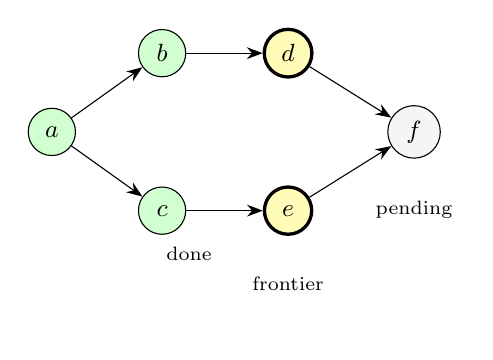
\begin{tikzpicture}[
  every node/.style = {circle, draw, minimum size=6mm, font=\small},
  done/.style  = {fill=green!18},
  fr/.style    = {fill=yellow!28, very thick},
  todo/.style  = {fill=gray!8},
  arr/.style   = {-{Stealth[length=2mm]}},
  >=Stealth,
]
\node[done] (a) at (0,0) {$a$};
\node[done] (b) at (1.4,1) {$b$};
\node[done] (c) at (1.4,-1) {$c$};
\node[fr]   (d) at (3,1) {$d$};
\node[fr]   (e) at (3,-1) {$e$};
\node[todo] (f) at (4.6,0) {$f$};
\draw[arr] (a)--(b); \draw[arr] (a)--(c);
\draw[arr] (b)--(d); \draw[arr] (c)--(e);
\draw[arr] (d)--(f); \draw[arr] (e)--(f);
\node[draw=none, font=\scriptsize, below right=0mm and -2mm of c] {done};
\node[draw=none, font=\scriptsize, below=0mm of e] {frontier};
\node[draw=none, font=\scriptsize, below=0mm of f] {pending};
\end{tikzpicture}
\end{center}

In this fragment, $\{a,b,c\}$ are completed, $\{d,e\}$ are on the frontier,
and $f$ is still waiting on its prerequisites. The frontier diamond
property says $d$ and $e$ can be executed in either order with the same
result.

% =====================================================================
\section{Machines}

An event graph is a static description; a \DefRef{Machine} is the
abstract asynchronous execution carrier into which it is interpreted.

\subsection{The machine carrier}
\label{def:Machine}

\begin{leanbox}
structure Machine (Player : Type) where\\
\bd State    : Type\\
\bd Action   : Player $\to$ Type\\
\bd Internal : Type\\
\bd Public   : Type\\
\bd Obs      : Player $\to$ Type\\
\bd Outcome  : Type\\[2pt]
\bd init    : State\label{def:init}\\
\bd available         : State $\to$ (p : Player) $\to$ Set (Action p)\label{def:available}\\
\bd availableInternal : State $\to$ Set Internal\label{def:availableInternal}\\
\bd stepPlay     : (p : Player) $\to$ Action p $\to$ State $\to$ PMF State\label{def:stepPlay}\\
\bd stepInternal : Internal $\to$ State $\to$ PMF State\label{def:stepInternal}\\[2pt]
\bd terminal   : State $\to$ Prop\label{def:terminal}\\
\bd publicView : State $\to$ Public\label{def:publicView}\\
\bd observe    : (p : Player) $\to$ State $\to$ Obs p\label{def:observe}\\
\bd outcome    : State $\to$ Outcome\label{def:outcome}\\
\bd utility    : Outcome $\to$ Payoff Player\label{def:utility}
\end{leanbox}

A machine is a tuple
\[
\begin{aligned}
  M \;=\; \bigl(\;
    & S,\; \{A_p\}_p,\; I,\; \mathrm{Pub},\; \{O_p\}_p,\; \Outcome,\;
       s_0, \\
    & \mathrm{avail},\; \mathrm{availInt},\;
       \mathrm{stepPlay},\; \mathrm{stepInternal},\;
       \mathrm{term},\; \mathrm{pubView},\; \mathrm{obs},\; \mathrm{out},\; u
  \;\bigr),
\end{aligned}
\]
where $u : \Outcome \to (\Players \to \mathbb{R})$. A primitive
\emph{event} is either $(\mathsf{play}, p, a)$ for $a \in A_p$ or
$(\mathsf{internal}, e)$ for $e \in I$; the combined transition kernel
$\mathrm{step}_M : \mathrm{Event}_M \times S \to \PMF S$ is total.

\paragraph{Total step, separate availability.}
$\TT{stepPlay}$ and $\TT{stepInternal}$ are total functions; legality
of an event is a \emph{separate} predicate. The event-graph machine
instance below implements a \emph{stuttering} convention — unavailable
events leave the state unchanged, returning $\mathrm{PMF.pure}\,s$. The
abstract \DefRef{Machine} carrier does not pre-commit to that
convention; the kernel is exposed unconstrained so backends can choose
their reaction.

\subsection{Run prefixes, schedulers, traces}

\begin{leanbox}
structure RunPrefix (M : Machine Player) where\label{def:RunPrefix}\\
\bd events : List M.Event\\
\bd states : List M.State\\
\bd length\_eq : states.length = events.length + 1\\[3pt]
abbrev EventLaw (M : Machine Player) : Type :=\label{def:EventLaw}\\
\bd M.State $\to$ PMF M.Event\\[3pt]
def IsLegalEventLaw (M : Machine Player) (law : M.EventLaw) : Prop :=\label{def:IsLegalEventLaw}\\
\bd $\forall$ s, $\neg$ M.terminal s $\to$ $\forall$ \{e\},\\
\bdd e $\in$ (law s).support $\to$ M.EventAvailable s e
\end{leanbox}

A \DefRef{RunPrefix} pairs a list of $n$ events with a list of $n+1$
states. An \DefRef{EventLaw} is a history-independent scheduler
$\lambda : S \to \PMF{\mathrm{Event}}$ choosing the next event from a
state; \DefRef{IsLegalEventLaw} requires the law to put mass only on
currently available events at non-terminal states. Iterating a legal
law for $n$ steps from $s_0$ yields a distribution over
$\mathrm{Tr}_n(M)$ — finite event-state traces of length $n$.
Marginalising on the final state and projecting via $\mathrm{out}$
gives the outcome kernel $\mathrm{outcomeKernelFrom}_\lambda$.

\subsection{The event-graph machine interpretation}

For an event graph $G$, the machine instance takes
\[
  \TT{State} := \DefRef{Configuration}\,G,
  \quad
  \TT{Action}\,p := \TT{PlayerAction}\,G\,p,
  \quad
  \TT{Internal} := \TT{InternalEvent}\,G.
\]
A $\TT{PlayerAction}\,G\,p$ is a pair $(n, \mathrm{slice})$ with $n :
G.\TT{Node}$ and $\mathrm{slice} : G.\TT{WriteSlice}$; availability
restricts it to frontier nodes owned by $p$ with a legal slice.
Internal events are $\TT{InternalEvent.node}\,n$ for non-player
frontier nodes, plus an always-unavailable
\DefRef{idle}\label{def:idle} constructor.

Reading $G$ as a machine, an event is the execution of one frontier
node. $\TT{stepPlay}$ stutters on unavailable actions (returns
$\mathrm{PMF.pure}\,\mathrm{cfg}$) and otherwise commits the chosen
slice. The diamond property and frontier-read stability lemmas
(\DefRef{withResult_comm}\label{def:withResult_comm} and companions)
provide the algebraic foundation for the round-based presentations of
\S\ref{sec:round-fosg}.

\paragraph{Stable frontier rounds: \TT{HasStableFrontierRounds}.}
\label{def:stableFrontier}
The lift from machine to FOSG requires the graph to satisfy
\DefRef{HasStableFrontierRounds}\label{def:HasStableFrontierRounds},
which combines two conditions:
\begin{itemize}\itemsep1pt
\item \emph{Existence.} Every player-owned frontier node has at least
  one available player action
  (\DefRef{HasAvailablePlayerActions}\label{def:HasAvailablePlayerActions}).
\item \emph{Stability.} If an action $a$ for player $p$ is available
  at $\mathrm{cfg}$ and $a.\TT{node}$ is on the frontier with
  $a.\TT{node} \neq \TT{first}$, then after legally executing any
  other frontier node $\TT{first}$, $a$ remains available.
\end{itemize}
Without stability, two players' frontier choices could race — one
execution could invalidate the other's still-pending action — and
round-level batching would be ill-defined. Vegas's source-elaborated
event graphs satisfy this predicate; a generic backend graph need not.

% =====================================================================
\section{Native Round and FOSG Views}
\label{sec:round-fosg}

The shift from machine to game-theoretic structure now happens through the
native \TT{Machine.RoundView}\label{def:Machine.RoundView}.  The FOSG view is the parallel
presentation used to reuse the GameTheory FOSG, EFG, and Kuhn machinery.

\subsection{Bounded states}

\paragraph{Lean.}
\TT{structure BoundedState (M : Machine P) (horizon : Nat) where state, depth, depth_le}.

\paragraph{Math.}
A \emph{bounded state} pairs a machine state with a depth counter, used to
present finite-horizon native round and FOSG views. The counter is
presentation data — the underlying machine state remains semantic.

\subsection{The native round view: \TT{Machine.RoundView}}
\label{def:RoundView}

\paragraph{Lean.}
\TT{structure RoundView (M : Machine P) where}
\begin{quote}
\TT{Act : P} $\to$ \TT{Type} \\
\TT{active : M.State} $\to$ \TT{Finset P} \\
\TT{availableActions : M.State} $\to$ \TT{(p : P)} $\to$ \TT{Set (Act p)} \\
\TT{transition : (state : M.State)} $\to$
  \TT{ \{a : JointAction Act //}
  \TT{ JointActionLegal Act active M.terminal availableActions state a\}} $\to$
  \TT{PMF M.State} \\
\TT{eventBlock : M.State} $\to$ \TT{JointAction Act} $\to$ \TT{List M.Event} \\
(\TT{terminal_active_eq_empty}, \TT{nonterminal_exists_legal})
\end{quote}

\paragraph{Math.}
\TT{RoundView} is the Vegas-facing strategic view of a machine.  It packages
round-action alphabets, active sets, available actions, the round transition,
and the primitive event block represented by a round.  Its bounded histories,
reachable information states, legal pure strategies, legal PMF-behavioral
strategies, and outcome kernels are defined in \TT{Vegas/Machine/RoundView.lean}
without importing FOSG.

\subsection{The FOSG view: \TT{Machine.FOSGView}}
\label{def:FOSGView}\label{def:Machine.FOSGView}

\paragraph{Lean.}
\TT{structure FOSGView (M : Machine P) where}
\begin{quote}
\TT{Act : P} $\to$ \TT{Type} \\
\TT{active : M.State} $\to$ \TT{Finset P} \\
\TT{availableActions : M.State} $\to$ \TT{(p : P)} $\to$ \TT{Set (Act p)} \\
\TT{transition : (state : M.State)} $\to$
  \TT{ \{a : JointAction Act //}
  \TT{ JointActionLegal Act active M.terminal availableActions state a\}} $\to$
  \TT{PMF M.State} \\
\TT{reward : (src : M.State)} $\to$
  \TT{ \{a : JointAction Act //}
  \TT{ JointActionLegal Act active M.terminal availableActions src a\}} $\to$
  \TT{M.State}\label{def:M.State} $\to$ \TT{P} $\to$ $\mathbb{R}$ \\
(\TT{terminal_active_eq_empty}\label{def:terminal_active_eq_empty}, \TT{nonterminal_exists_legal}\label{def:nonterminal_exists_legal})
\end{quote}

\paragraph{Math.}
A \emph{factored-observation stochastic game view} on top of a machine is
the FOSG presentation counterpart of the native round view: at each state, a
finite set of \emph{active} players choose round-actions from \TT{Act}\label{def:Act}, the state transitions
stochastically, and a per-player reward is paid out at the transition.
Crucially, the round-action alphabet \TT{Act} is independent of the
machine action alphabet \TT{M.Action}\label{def:M.Action}: a single round may consist of many
machine events. For event-graph protocols, a \TT{PlayerRoundAction}\label{def:PlayerRoundAction}
is a total assignment of candidate slices to graph nodes; the round menu
uses only the coordinates for the player's owned current-frontier nodes.

\paragraph{Round menus and observation equivalence.}
For event-graph machines the player-facing menu at a frontier round is packaged
as \TT{EventGraph.roundMenu G cfg who}: a set of optional round-actions
where \texttt{none} means the player is not active in the current round and
\texttt{some action} means the player is active and \texttt{action}'s relevant
coordinates are legal on every current frontier node they own. Irrelevant
coordinates of the total slice assignment are ignored. The accompanying theorem
\TT{eventGraph_roundMenu_eq_of_observation_eq}\label{def:eventGraph_roundMenu_eq_of_observation_eq} shows that two configurations
that are indistinguishable to a player offer that player the same menu —
the structural form of ``a player's available choices depend only on what
they observe.''

\paragraph{Why FOSG and not extensive form.}
Standard extensive-form games index strategies by histories; FOSG indexes
strategies by \emph{information sets}, which are equivalence classes of
histories under per-player observation. FOSG is a modern state-based
formalism that cleanly separates public and private observation; the
GameTheory submodule of this project formalizes FOSGs once and Vegas wires
its machine semantics into the existing carrier.

\subsection{The canonical EFG presentation}

\paragraph{Lean.}
\TT{Vegas/GameBridge/EFG/FromEventGraph.lean} applies GameTheory's
\TT{FOSG.AugmentedEFGBridge}\label{def:FOSG.AugmentedEFGBridge} to the bounded program event-graph FOSG:
\begin{quote}
\TT{eventGraphEFGAt g : EFG.EFGGame} \\
\TT{eventGraphEFGBehavioralProfileAt g beta} \\
\TT{eventGraphEFGAt_outcomeKernel_map_publicOutcome}\label{def:eventGraphEFGAt_outcomeKernel_map_publicOutcome}
\end{quote}
The bridge tree is not a hand-written textbook tree. It is the canonical
serialisation of one FOSG round: one EFG decision opportunity per player
(over optional local moves), followed by a chance node for the FOSG
transition. Translated legal FOSG strategies put all mass on \TT{none} for
inactive players, so these administrative decision opportunities do not add
strategic freedom.

\paragraph{Tree structure, not only distributions.}
The semantic adequacy theorem says that projecting EFG terminal histories
back to public Vegas outcomes gives the same outcome law as the bounded
event-graph FOSG behavioral presentation.  The native/FOSG equivalence
theorems in \TT{GameBridge/FOSG/NativeEquiv.lean} transport this law to
\TT{pmfBehavioralKernelGameAt}\label{def:pmfBehavioralKernelGameAt}; the named EFG theorem itself is still
stated at the FOSG presentation boundary. For reviewers who want to see the actual tree spine,
\TT{EFG.GameTree.HasDecisionChainThenChance}\label{def:EFG.GameTree.HasDecisionChainThenChance} records the
structural predicate ``$n$ sequential decisions followed by chance''. The
example file \TT{Examples/EFGTranslation.lean} proves this predicate for the
first generated round of the checked examples. Thus the code now checks both
the law induced by the EFG and the expected root shape of the generated tree.

\subsection{Bounded FOSGs and outcome kernels}

\paragraph{Math.}
\TT{toBoundedFOSG horizon} wraps a FOSG view in \TT{BoundedState}\label{def:BoundedState} so that
games are presented with a strict horizon — a hard prerequisite for many of
the finite-game theorems imported from the GameTheory library. The bounded
view exposes outcome kernels
\[
  \mathrm{outcomeFromPure}_h\,\pi : \PMF{\Outcome\,M},
  \qquad
  \mathrm{outcomeFromBehavioral}_h\,\beta : \PMF{\Outcome\,M},
\]
from pure and behavioral profiles respectively. The horizon $h$ is fixed
by the program: \TT{syntaxSteps} (\TT{Vegas/Core/Config.lean}) counts every
source constructor except \Ret, including administrative \Let{}s. The depth
counter in \TT{BoundedState} is presentation data needed to prove the
\emph{FOSG tree's} finiteness; the underlying event graph is already finite, but
without bounding the FOSG presentation could in principle re-visit
configurations.

\paragraph{Round-batching diagram.}
\begin{center}
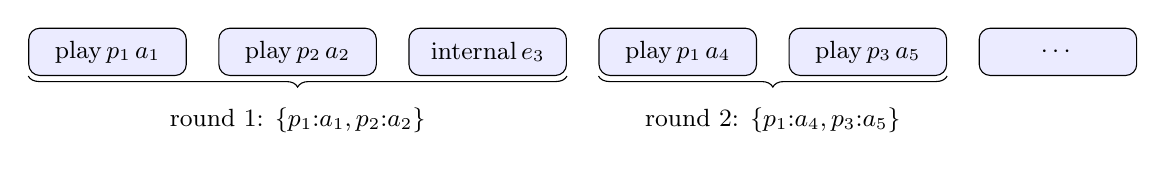
\begin{tikzpicture}[
  node distance=4mm,
  ev/.style = {draw, rounded corners, fill=blue!8, font=\small,
    minimum height=6mm, minimum width=20mm},
  arr/.style = {-{Stealth[length=2mm]}, thick},
  bra/.style = {decorate, decoration={brace, amplitude=4pt, mirror}},
]
\node[ev] (e1) {$\mathrm{play}\,p_1\,a_1$};
\node[ev, right=of e1] (e2) {$\mathrm{play}\,p_2\,a_2$};
\node[ev, right=of e2] (e3) {$\mathrm{internal}\,e_3$};
\node[ev, right=of e3] (e4) {$\mathrm{play}\,p_1\,a_4$};
\node[ev, right=of e4] (e5) {$\mathrm{play}\,p_3\,a_5$};
\node[ev, right=of e5] (edots) {$\cdots$};
\draw[bra] (e1.south west) -- (e3.south east)
  node[midway, below=8pt, font=\small] {round 1: $\{p_1{:}a_1, p_2{:}a_2\}$};
\draw[bra] (e4.south west) -- (e5.south east)
  node[midway, below=8pt, font=\small] {round 2: $\{p_1{:}a_4, p_3{:}a_5\}$};
\end{tikzpicture}
\end{center}

\noindent The machine is the bottom layer (every primitive event explicit);
the native round view turns the current frontier into a single strategic
round by executing \TT{cfg.frontier.toList}.  The FOSG view mirrors that same
round as a presentation for the GameTheory FOSG infrastructure. Player-owned
nodes read the selected round-action slices, and internal nodes use their
event-graph kernels. Nodes newly enabled while this list runs are left for a
later round. The stability predicate of \S\ref{def:stableFrontier} and the
frontier linearisation theorem are what make this presentation independent of
strategically irrelevant scheduling choices.

% =====================================================================
\section{The Strategic API}
\label{sec:strategic}

For a checked program $g$, the codebase exposes a public API of strategy
spaces, game forms, and kernel games.

\subsection{Strategies and profiles}
\label{def:strategies}

\begin{leanbox}
def pureStrategyAt           (g : WFProgram P L) (p : P) : Type\\
def behavioralStrategyPMFAt  (g : WFProgram P L) (p : P) : Type\\
def pureProfileAt            (g : WFProgram P L)         : Type\\
def behavioralProfilePMFAt   (g : WFProgram P L)         : Type
\end{leanbox}

For each player $p$ the native round view (\DefRef{eventGraphRoundView}\label{def:eventGraphRoundView})
induces a finite
set of \emph{information states} $\mathcal{I}_p$: equivalence classes of
bounded native round histories under $p$'s observation. The strategic carrier uses a
\emph{reachability-pruned} version
\[
  \mathrm{ReachableInfoState}\,p \;=\;
    \bigl\{\, s \in \mathcal{I}_p \;\bigm|\;
      \exists\, h : \mathrm{History}.\; h.\mathrm{playerView}\,p = s\,\bigr\}
\]
— information states \emph{realised by some native bounded history}, not by
some \emph{positive-probability} profile run. (This is purely combinatorial
and avoids quantifying over profiles in the carrier definition.)

A pure strategy for $p$ is then
\[
  \mathrm{ReachablePureStrategy}\,p \;=\;
    \mathrm{ReachableInfoState}\,p \;\to\; \mathrm{Option}\,(\mathrm{Act}\,p),
\]
returning \texttt{none} at information states where $p$ is not active and
\texttt{some}\,$a$ at active ones. A \emph{behavioral strategy} is
\[
  \mathrm{ReachableBehavioralStrategy}\,p \;=\;
    \mathrm{ReachableInfoState}\,p \;\to\; \PMF{\mathrm{Option}\,(\mathrm{Act}\,p)}.
\]
The Vegas \emph{legal} carriers (\TT{LegalPureProfile}\label{def:LegalPureProfile},
\TT{LegalBehavioralProfile}\label{def:LegalBehavioralProfile}) further restrict the support: at any reachable
information state where $p$ is active, the chosen \texttt{some}\,$a$ must
satisfy $a \in \mathrm{availableMoves}\,p\,h$ for every native history $h$
realising that information state. \emph{This is what closes the gap from program-level \Legal{}
to strategic legality}: illegal moves are simply not in the strategy carrier
for the equilibrium predicates to range over.

\subsection{Game forms and kernel games}
\label{def:kernelgames}

The codebase exposes six game forms and four kernel games for a
checked program $g$, organised by strategy carrier and outcome shape.

\begin{leanbox}
-- payoff-vector outcomes\\
def pureGameFormAt                        g\label{def:pureGameFormAt}\\
def pmfBehavioralGameFormAt               g\label{def:pmfBehavioralGameFormAt}\\[2pt]
-- terminal public-state outcomes\\
def purePublicStateGameFormAt             g\label{def:purePublicStateGameFormAt}\\
def pmfBehavioralPublicStateGameFormAt    g\label{def:pmfBehavioralPublicStateGameFormAt}\\[2pt]
-- blocked-trace outcomes\\
def pureBlockedTraceGameFormAt            g\label{def:pureBlockedTraceGameFormAt}\\
def pmfBehavioralBlockedTraceGameFormAt   g\label{def:pmfBehavioralBlockedTraceGameFormAt}\\[3pt]
-- kernel games (game form + canonical utility)\\
def pureKernelGameAt                      g\label{def:Vegas.pureKernelGame}\\
def pmfBehavioralKernelGameAt             g\label{def:Vegas.pmfBehavioralKernelGame}\\
def pureBlockedTraceKernelGameAt          g\\
def pmfBehavioralBlockedTraceKernelGameAt g
\end{leanbox}


A \TT{GameTheory.GameForm}\label{def:GameTheory.GameForm} contains per-player strategy
types, an outcome type, and a stochastic kernel from profiles to outcomes.
A \TT{GameTheory.KernelGame}\label{def:GameTheory.KernelGame} adds a utility function. The payoff-vector
and blocked-trace game forms have canonical utilities and therefore produce
the four kernel games. The terminal-public-state forms intentionally stop at
the game-form level: they expose the final public observation as data, not a
payoff interpretation. The kernel games span two orthogonal axes:
\begin{itemize}\itemsep1pt
\item \emph{Strategy carrier}: pure vs.\ PMF-behavioral.
\item \emph{Outcome shape}: the payoff vector $\Outcome\,\Players$ versus
  the richer \texttt{syntaxBlockedTraceAt}\,$g$ which retains the per-round
  primitive-event blocks and their endpoint machine state.
\end{itemize}
The blocked-trace games refine the payoff-vector games by an outcome
projection, packaged as a kernel-game morphism (next subsection).

\paragraph{Unsuffixed APIs.}
The unsuffixed names \TT{Vegas.pureGameForm},
\TT{Vegas.purePublicStateGameForm}, \TT{Vegas.pureKernelGame},
\TT{Vegas.pmfBehavioralGameForm},
\TT{Vegas.pmfBehavioralPublicStateGameForm}, and
\TT{Vegas.pmfBehavioralKernelGame} are thin definitions equal to their
\TT{*At} counterparts under \TT{[Fintype P]} and \TT{[FiniteDomains
g]}; they are definitionally equal, so all theorems transport.

\subsection{The kernel-game carrier}
\label{def:KernelGame}

\begin{leanbox}
structure KernelGame ($\Players$ : Type) where\\
\bd Strategy      : $\Players$ $\to$ Type\\
\bd Outcome       : Type\label{def:Outcome}\\
\bd utility       : Outcome $\to$ Payoff $\Players$\label{def:Payoff}\\
\bd outcomeKernel : Kernel ($\Pi$ i, Strategy i) Outcome
\end{leanbox}

A \emph{kernel game} is the minimal object on top of which all
expected-utility solution concepts can be defined:
\[
\KG \;=\; \bigl(\{S_p\}_p,\,O,\,
  K : \textstyle\prod_p S_p \to \PMF{O},\;
  u : O \to \mathrm{Payoff}\,\Players\bigr),
\]
where the payoff vector type is
$\mathrm{Payoff}\,\Players = \Players \to \mathbb{R}$. Expected utility
is
\[
  \EU(\sigma, p) \;=\;
    \mathbb{E}_{\omega \sim K(\sigma)}\bigl[u(\omega)(p)\bigr].
\]
Splitting $K$ from $u$ separates \emph{protocol}
(\DefRef{GameForm}\label{def:GameForm}) from \emph{preference}, which
is what enables the preference-parameterised solution concepts of the
next subsection.

\paragraph{Outcome types in the codebase.}
Vegas's protocol-level outcome is
$\Outcome\,\Players = \Players \to_0 \mathbb{Z}$
(\S\ref{sec:outcomes}). The payoff-vector kernel games
\DefRef{pureKernelGameAt}\label{def:pureKernelGameAt} and
\TT{pmfBehavioralKernelGameAt} take $O = \Outcome\,\Players$ and use
the coercion $u(o)(p) = (o\,p : \mathbb{R})$. The public-state game
forms set $O$ to the terminal \TT{ProgramPublicObs}\,$g$ and have no
canonical utility. The blocked-trace games set $O$ to
\[
  \mathtt{syntaxBlockedTraceAt}\,g \;=\;
    [\![\mathrm{event\ blocks}]\!] \times \mathtt{State}_M,
\]
each native round's primitive-event block paired with the round's
endpoint machine state, with utility
$\mathrm{tr} \mapsto u_{\mathrm{public}}(\mathrm{out}(\mathrm{tr}.\TT{state}))$.

\paragraph{Refinement layer.}
The relationship between the blocked-trace and payoff-vector games is
packaged as a
\DefRef{KernelGame.Simulation}\label{def:KernelGame.Simulation} —
definitionally a \DefRef{Morphism}\label{def:Morphism} preserving the
joint utility-distribution $\mathrm{udist}$ over payoff vectors under
profile mapping. Explicit expected-utility-equality lemmas
\DefRef{pureBlockedTraceKernelGameAt_eu_eq}\label{def:pureBlockedTraceKernelGameAt_eu_eq}
and its behavioural counterpart, plus the symmetric
\DefRef{Bisimulation}\label{def:Bisimulation} and
\DefRef{EUBisimulation}\label{def:EUBisimulation} objects, certify that
reasoning at either game level is sound: outcome projection preserves
utility distributions, and EU is provably equal across the projection.

\subsection{Linear source reading}
\label{def:LinearRead}

\begin{leanbox}
def syntaxLinearRead (g : WFProgram P L) : List (ProgramNode g) :=\\
\bd ProgramNode.enumerate g.prog\\[3pt]
theorem syntaxLinearRead\_sufficient :\\
\bd $\forall$ (cfg : Configuration (programEventGraph g)),\\
\bd \ \ $\neg$ cfg.terminal $\to$\\
\bd \ \ $\exists$ n $\in$ syntaxLinearRead g,\\
\bd \ \ \ \ n.rank-minimal $\land$ on-frontier cfg
\end{leanbox}

The source-order rank on
\DefRef{ProgramNode}\label{def:ProgramNode}s is a topological order
for the elaborated event graph: every prerequisite of a node has
strictly smaller rank. A reader who scans the program in rank order
and stops at the first unfinished source event therefore lands on an
event whose dependencies are already complete. Event-graph executions
may take independent frontier nodes in other orders, but the
straight-line source presentation never blocks early. The reusable
event-graph-level theorem is
\DefRef{EventGraph.Configuration.exists_rank_minimal_enabled_of_not_terminal}\label{def:EventGraph.Configuration.exists_rank_minimal_enabled_of_not_terminal}.

\paragraph{Commit/reveal information barrier.}
Three theorems state that an earlier commit and a reveal of that
commit cannot be frontier-simultaneous, and that the corresponding
player action is unavailable while the reveal is on the frontier:
\begin{itemize}\itemsep0pt
\item \DefRef{eventGraph_priorCommit_not_frontier_with_reveal}\label{def:eventGraph_priorCommit_not_frontier_with_reveal} — the graph-level statement.
\item \DefRef{reveal_not_frontier_with_prior_commit}\label{def:reveal_not_frontier_with_prior_commit} — its program-facing wrapper.
\item \DefRef{prior_commit_not_available_when_reveal_frontier}\label{def:prior_commit_not_available_when_reveal_frontier} — the strategy-surface corollary.
\end{itemize}
This is the theorem-level guard against observing a reveal before
choosing an earlier same-phase commitment.

\paragraph{Role.}
Source order is a readable topological schedule for the dependency
graph: following it never gets stuck before the event graph is
terminal. Strategic equivalence across stable frontier schedules is
then proved by the frontier-stability, blocked-trace, and morphism
layers.

\subsection{Solution concepts (Vegas-facing definitions)}
\label{def:solution}\label{def:IsNash}\label{def:IsStrictNash}\label{def:WeaklyDominates}\label{def:StrictlyDominates}\label{def:IsCorrelatedEq}\label{def:IsCoarseCorrelatedEq}\label{def:ParetoDominates}\label{def:IsParetoEfficient}\label{def:socialWelfare}\label{def:IsExactPotential}\label{def:IsOrdinalPotential}\label{def:IsZeroSum}\label{def:IsConstantSum}\label{def:IsTeamGame}\label{def:optimalWelfare}\label{def:bestNashWelfare}\label{def:worstNashWelfare}\label{def:worstNashWelfare_le_bestNashWelfare}\label{def:bestNashWelfare_le_optimalWelfare}\label{def:ciSup}

The Vegas definitions
(\DefRef{Vegas.IsNash}\label{def:Vegas.IsNash},
\DefRef{IsBestResponse}\label{def:IsBestResponse},
\DefRef{IsDominant}\label{def:IsDominant}, \ldots) are thin wrappers
around GameTheory's preference-parameterised predicates over the
PMF-behavioural kernel game \TT{pmfBehavioralKernelGame g}. They cover
Nash, dominance, correlated and coarse-correlated equilibria, social
welfare, approximate Nash, potentials, and constant-sum/team
properties. For each, the Lean wrapper has the form
$\TT{Vegas.}X = (\DefRef{pmfBehavioralKernelGame}\label{def:pmfBehavioralKernelGame}\,g).X$.
We use $\EU(\sigma, p)$ for expected utility.

\smallskip
\noindent\begin{tabular}{@{}lp{0.55\textwidth}@{}}
\toprule
\textbf{Predicate} & \textbf{Mathematical content (over $\KG$, $\sigma : \Pi_p S_p$)} \\
\midrule
\DefRef{IsNash}~$\sigma$ &
  $\forall p,\, \forall s'_p \in S_p.\; \EU(\sigma, p) \ge \EU(\sigma[p \mapsto s'_p], p)$. \\
\DefRef{IsStrictNash}~$\sigma$ &
  As above with $>$ for $s'_p \neq \sigma_p$. \\
\DefRef{IsBestResponse}~$p\,\sigma\,s$ &
  $\forall s'.\; \EU(\sigma[p\mapsto s], p) \ge \EU(\sigma[p\mapsto s'], p)$. \\
\DefRef{IsDominant}~$p\,s$ &
  $\forall \sigma\, s'.\; \EU(\sigma[p\mapsto s], p) \ge \EU(\sigma[p\mapsto s'], p)$. \\
\DefRef{WeaklyDominates}~$p\,s\,t$ &
  $\forall \sigma_{-p}.\, \EU((s, \sigma_{-p}), p) \ge \EU((t, \sigma_{-p}), p)$. \\
\DefRef{StrictlyDominates}~$p\,s\,t$ &
  As above with $>$. \\
\DefRef{IsCorrelatedEq}~$\mu$ &
  Profile distribution $\mu$: no recommendation-dependent unilateral
  deviation strictly improves any player's outcome distribution. \\
\DefRef{IsCoarseCorrelatedEq}~$\mu$ &
  As above, restricted to constant deviations. \\
\DefRef{ParetoDominates}~$\sigma\,\tau$ &
  $\forall p.\,\EU(\sigma, p) \ge \EU(\tau, p)$ and $\exists p.\,>$. \\
\DefRef{IsParetoEfficient}~$\sigma$ &
  $\nexists \tau.\; \mathrm{ParetoDominates}\,\tau\,\sigma$. \\
\DefRef{socialWelfare}~$\sigma$ &
  $\sum_p \EU(\sigma, p)$. \\
\DefRef{IsExactPotential}~$\Phi$ &
  $\Phi : \Pi_p S_p \to \mathbb{R}$ such that
  $\Phi(\sigma[p\!\mapsto\!s']) - \Phi(\sigma) = \EU(\sigma[p\!\mapsto\!s'], p) - \EU(\sigma, p)$. \\
\DefRef{IsOrdinalPotential}~$\Phi$ &
  Sign-only version. \\
\DefRef{IsZeroSum}, \DefRef{IsConstantSum}~$c$ &
  $\sum_p u(\omega)(p)$ is constant ($=0$ or $=c$) on all outcomes. \\
\DefRef{IsTeamGame} &
  $u(\omega)(p) = u(\omega)(q)$ for all $p, q, \omega$. \\
\texttt{Is}$\varepsilon$\texttt{Nash}~$\sigma$ &
  $\forall p\, s'_p.\, \EU(\sigma, p) + \varepsilon \ge \EU(\sigma[p\mapsto s'_p], p)$. \\
\DefRef{optimalWelfare} &
  $\sup_\sigma \mathrm{socialWelfare}(\sigma)$ (via \DefRef{ciSup};
  finite-profile variants are picked up by Mathlib's boundedness
  lemmas). Vegas also defines
  \DefRef{bestNashWelfare} and \DefRef{worstNashWelfare}, with
  comparison lemmas
  \DefRef{worstNashWelfare_le_bestNashWelfare} and
  \DefRef{bestNashWelfare_le_optimalWelfare}. \\
\bottomrule
\end{tabular}

\paragraph{Preference parameterisation.}
GameTheory exposes $\TT{IsNashFor}\,\TT{pref}$,
$\TT{IsBestResponseFor}\,\TT{pref}$, etc., where
\DefRef{pref}\label{def:pref} is an arbitrary preference relation over
$\PMF\Outcome$. The Vegas-named EU versions arise by instantiating
$\mathtt{pref} = \mathtt{euPref}$ (expected-value comparison).

\paragraph{Existence corollaries.}
Three finite-game existence theorems are exposed through the
Vegas-facing API as direct wrappers of the GameTheory fixed-point and
correlated-equilibrium existence results, instantiated at
\TT{pmfBehavioralKernelGame g}:
\DefRef{mixedNash_exists}\label{def:mixedNash_exists},
\DefRef{correlatedEq_exists}\label{def:correlatedEq_exists}, and
\DefRef{coarseCorrelatedEq_exists}\label{def:coarseCorrelatedEq_exists}.
They are stated at the PMF-over-strategies level and do not themselves
construct a named source-level policy.

\subsection{Mixed extension and Kuhn realisation}
\label{def:Kuhn}

\begin{leanbox}
def KernelGame.mixedExtension (G : KernelGame $\Players$) : KernelGame $\Players$\\[3pt]
theorem NativeFOSG.boundedOutcomeFromBehavioral\_nativeToFOSG\label{def:boundedOutcomeFromBehavioral_nativeToFOSG}\\
theorem NativeFOSG.boundedOutcomeFromPure\_nativeToFOSG\label{def:boundedOutcomeFromPure_nativeToFOSG}\\[3pt]
theorem kuhn\_finiteKernelGame\label{def:kuhn_finiteKernelGame}\\
theorem Vegas.kuhn\_finite\label{def:Vegas.kuhn_finite}
\end{leanbox}

The \emph{mixed extension} of a finite kernel game $\KG$ replaces each
strategy space $S_p$ by $\PMF S_p$. The outcome kernel of the extension
samples $\sigma \sim \prod_p \mu_p$ from the independent product
distribution and applies the underlying kernel:
\[
  K^{\mathrm{mix}}(\mu) \;=\; \bigl(\textstyle\prod_p \mu_p\bigr)
    \bind \lambda \sigma. K(\sigma).
\]

\emph{Kuhn realisation} for finite Vegas programs (\TT{kuhn_finite}\label{def:kuhn_finite}): every
independent mixed profile over the pure strategy carrier of
\TT{pureKernelGameAt}$\,g$ is matched by a behavioral profile of
\TT{pmfBehavioralKernelGameAt}$\,g$ with the \emph{same payoff-vector
outcome distribution}. Symbolically, with $\KG^{\mathrm{pure}}$ and
$\KG^{\mathrm{beh}}$ the two kernel games:
\[
  \forall \mu \in \textstyle\prod_p \PMF{S_p^{\mathrm{pure}}}.\;\;
  \exists \beta : \mathrm{Profile}(\KG^{\mathrm{beh}}).\;\;
    K^{\mathrm{beh}}(\beta) \;=\;
    \bigl(\textstyle\prod_p \mu_p\bigr) \bind K^{\mathrm{pure}}.
\]

\paragraph{Hypotheses behind the slogan.}
The Lean statement is a Kuhn-style realisation theorem, not merely the
textbook phrase ``perfect recall'' copied verbatim. The unconditional theorem
is routed through the bounded FOSG view of the program event-graph machine:
finite domains provide the finite-horizon FOSG carriers, and the required
information condition is \TT{LegalObservable}\label{def:LegalObservable} for the bounded FOSG, proved for
checked program event graphs from the visibility and graph-stability
invariants. The public native theorem transports the FOSG realization through the proved
native/FOSG equivalence: native pure profiles map to FOSG pure profiles,
native behavioral profiles have the same bounded outcome law after transport,
and pure-to-behavioral outcome laws agree on both sides.

\paragraph{Why this is the headline theorem.}
Pure strategies are easy to read and define; behavioral strategies are
what equilibrium analyses on extensive-form games actually use. The Kuhn
realisation says that for every mixture over the simple objects we can
build a behavioral-profile witness with identical observable behavior.
This is the formal contract between the surface API (\TT{pureKernelGame}\label{def:pureKernelGame})
and the analysis API (\TT{pmfBehavioralKernelGame}).

\subsection{Finite pure kernel-game export}
\label{def:KernelGameExport}

\begin{leanbox}
structure KernelGameExport ($\Players$ : Type) where ...\label{def:KernelGameExport.structure}\\[3pt]
def KernelGameExport.ofKernelGame ...\label{def:KernelGameExport.ofKernelGame}\\
def pureKernelGameExport ...\label{def:pureKernelGameExport}\\
def pureBlockedTraceKernelGameExport ...\label{def:pureBlockedTraceKernelGameExport}
\end{leanbox}

\DefRef{KernelGameExport.structure} packages a finite pure kernel game
as the ingredients a solver adapter needs: the original player and
strategy types, finite lists of players and strategies, an
outcome-kernel oracle, and a utility function. It is an API boundary,
not a file format. It does not enumerate PMF-behavioural strategies,
whose carrier contains probability-valued functions, nor does it
provide a universal finite list of payoff-vector outcomes. Adapters to
Gambit, PRISM-games, or another solver are separate code building on
this object or on the canonical EFG presentation.

% =====================================================================
\section{Outcome and utility evaluation}
\label{sec:outcomes}

\subsection{Outcomes: \TT{Outcome}, \TT{mkOutcome}, \TT{evalPayoffs}}

\begin{leanbox}
abbrev Outcome (P : Type) [DecidableEq P] := P $\to_0$ $\mathbb{Z}$\\[3pt]
def mkOutcome (entries : List (P $\times$ Int)) : Outcome P\\[3pt]
def evalPayoffs\\
\bd (payoffs : List (P $\times$ L.Expr (erasePubVCtx $\Gamma$) L.int)) :\\
\bd VEnv L $\Gamma$ $\to$ Outcome P
\end{leanbox}

A protocol \emph{outcome} is a finitely-supported $\mathbb{Z}$-valued
payoff vector indexed by players,
$\Outcome\,\Players = \Players \to_0 \mathbb{Z}$.
\DefRef{mkOutcome}\label{def:mkOutcome} sums duplicate keys; absent
players default to payoff $0$.
\DefRef{evalPayoffs}\label{def:evalPayoffs} takes a \Ret{} node's
syntactic payoff list, evaluates each integer expression in the
public-erased environment, and packages the result.

\paragraph{Why \TT{Finsupp}, not \TT{P}~$\to$~\TT{Int}.}
\DefRef{Finsupp}\label{def:Finsupp} is decidably equal and decidably
has-zero — both of which are needed for $\PMF{\Outcome}$ to
type-check. The semantics of ``only named players are paid'' is the
same either way.

% =====================================================================
\section{The Backend Layer (refinement)}
\label{def:Backend}

\subsection{Refinement relations}

Both refinement structures carry projection data and an
initial-state-preservation obligation:
\begin{leanbox}
-- common projection fields\\
\bd projectState   : Impl.State $\to$ Spec.State\label{def:projectState}\\
\bd projectEvent   : Impl.Event $\to$ Option Spec.Event\label{def:projectEvent}\\
\bd projectPublic  : Impl.Public $\to$ Spec.Public\label{def:projectPublic}\\
\bd projectObs     : (p : P) $\to$ Impl.Obs p $\to$ Spec.Obs p\label{def:projectObs}\\
\bd projectOutcome : Impl.Outcome $\to$ Spec.Outcome\label{def:projectOutcome}\\
\bd init\_project  : projectState Impl.init = Spec.init\label{def:init_project}
\end{leanbox}

\begin{leanbox}
structure WeakStepRefinement (Impl Spec : Machine P) extends \ldots where\\
\bd external\_step\_sound\label{def:external_step_sound}\\
\bd internal\_step\_projectState\_eq\label{def:internal_step_projectState_eq}\\
\bd publicView\_project\label{def:publicView_project}\\
\bd observe\_project\label{def:observe_project}\\
\bd terminal\_project\label{def:terminal_project}\\
\bd terminal\_outcome\_projected\label{def:terminal_outcome_projected}\\[3pt]
structure StochasticStepRefinement (Impl Spec : Machine P) extends \ldots where\label{def:StochasticStepRefinement}\\
\bd step\_project\label{def:step_project}\\
\bd publicView\_project,\ observe\_project,\ terminal\_project\\
\bd terminal\_reflect\label{def:terminal_reflect}\\
\bd terminal\_outcome\_projected
\end{leanbox}

\emph{Refinement} is the verification-style relation: an implementation
is indistinguishable from a specification by any externally observable
behaviour. Concretely, a refinement is a state projection
$\pi : S_{\mathrm{Impl}} \to S_{\mathrm{Spec}}$ subject to matching
conditions on transitions. Two strengths are formalised:
\begin{itemize}\itemsep1pt
\item \emph{Weak step refinement.} Implementation player events match a
  specification event under the projection; internal events preserve
  the projected state.
\item \emph{Stochastic step refinement.} The strictly stronger version:
  the pushforward of the implementation step kernel through the
  projection equals the specification's kernel (with internal events
  stuttering on the spec side). This implies weak refinement
  (\DefRef{StochasticStepRefinement.toWeakStepRefinement}\label{def:StochasticStepRefinement.toWeakStepRefinement}).
\end{itemize}
Every machine refines itself
(\DefRef{StochasticStepRefinement.refl}\label{def:StochasticStepRefinement.refl});
the identity refinement serves both as a baseline backend and as a
compact smoke test for trace-projection theorems.

\paragraph{Why a separate layer.}
Real-runtime implementations carry machinery (transactions, schedulers,
gossip) absent from the source language. Refinement attests that
reasoning at the FOSG/kernel-game level transports to an implementation
without growing a second ``implementation semantics'' inside the source
language. Trace-level projection lemmas
\DefRef{runEventsFrom_project_eq}\label{def:runEventsFrom_project_eq}
and
\DefRef{blockTraceDist_project_eq}\label{def:blockTraceDist_project_eq}
carry the refinement from primitive events to whole runs.

\subsection{Backend kernel-game transport}

A \DefRef{StochasticStepRefinement} packages into a kernel-game
morphism via the following data:

\begin{leanbox}
structure PureSpecBlockLaw (g : WFProgram P L) where ...\label{def:PureSpecBlockLaw}\\
structure BehavioralSpecBlockLaw (g : WFProgram P L) where ...\label{def:BehavioralSpecBlockLaw}\\[3pt]
structure BackendPureBlockLawLift (g) (R) where ...\label{def:BackendPureBlockLawLift}\\
structure BackendBehavioralBlockLawLift (g) (R) where ...\label{def:BackendBehavioralBlockLawLift}\\[3pt]
def backendBlockedTraceKernelGameAt ... : KernelGame P\label{def:backendBlockedTraceKernelGameAt}\\
def toBackendBlockedTraceMorphism ... : KernelGame.EUMorphism\label{def:toBackendBlockedTraceMorphism}\label{def:KernelGame.EUMorphism}
\end{leanbox}

\begin{itemize}\itemsep1pt
\item \DefRef{PureSpecBlockLaw}~$g$ is a per-pure-profile specification
  block law plus a proof that it reproduces the canonical
  \DefRef{pureBlockedTraceKernelGameAt}\label{def:pureBlockedTraceKernelGameAt}
  outcome kernel.
\item \DefRef{BehavioralSpecBlockLaw}~$g$ is the analogous package for
  PMF behavioural profiles.
\item \DefRef{BackendPureBlockLawLift}~$g~R$ pairs per-pure-profile
  block-laws — one for the spec graph machine, one for the
  implementation — proved compatible via
  \DefRef{R.BlockLawCompatible}\label{def:R.BlockLawCompatible}
  and tied to a sound specification law.
\item \DefRef{BackendBehavioralBlockLawLift}~$g~R$ is the analogous
  datum for PMF behavioural profiles.
\item \DefRef{backendBlockedTraceKernelGameAt} is a kernel game whose
  strategy spaces are the canonical Vegas pure strategies but whose
  outcomes are full implementation block-traces.
\item \DefRef{toBackendBlockedTraceMorphism} and its behavioural
  counterpart expose, for every refinement plus lift, a
  \DefRef{KernelGame.EUMorphism} in the direction
  \[
    \text{backend game} \;\longrightarrow\; \text{spec blocked-trace game},
  \]
  the direction needed to \emph{pull Nash equilibria back from the
  spec to the backend}.
\end{itemize}

A backend author supplies a \DefRef{StochasticStepRefinement} plus a
block-law lift and obtains an EU-preserving morphism from the
implementation into the canonical Vegas blocked-trace game. The
separation of \TT{PureSpecBlockLaw}/\TT{BehavioralSpecBlockLaw} from
backend lifts is needed because FOSG blocked traces are indexed by
bounded FOSG histories while machine block laws are indexed by machine
blocked traces — the code asks for the soundness proof rather than
treating the conversion as definitional. For the identity refinement,
\DefRef{PureSpecBlockLaw.identityBackendLift}\label{def:PureSpecBlockLaw.identityBackendLift}
and
\DefRef{BehavioralSpecBlockLaw.identityBackendLift}\label{def:BehavioralSpecBlockLaw.identityBackendLift}
reuse the same packaged soundness proof.

\paragraph{Transport proofs use the morphism API.}
The two public pullback theorems
\DefRef{backendBlockedTraceKernelGameAt_isNash_pullback}\label{def:backendBlockedTraceKernelGameAt_isNash_pullback}
and
\DefRef{backendPMFBehavioralBlockedTraceKernelGameAt_isNash_pullback}\label{def:backendPMFBehavioralBlockedTraceKernelGameAt_isNash_pullback}
are proved by applying
\DefRef{KernelGame.EUMorphism.nash_of_nash}\label{def:KernelGame.EUMorphism.nash_of_nash}.
The composed ``payoff-vector game to backend'' theorems first use
\DefRef{EUGameIsomorphism.nash_iff}\label{def:EUGameIsomorphism.nash_iff}
between payoff-vector and blocked-trace games, then the backend
morphism. The code thus exercises the same morphism-composition story
stated in the report rather than repeating expected-utility
calculations locally.

% =====================================================================
\section{Worked Examples}

The codebase contains checked game examples, constructor-level smoke tests,
and backend/refinement examples. We summarise the textbook games first, then
the files whose purpose is to exercise API surfaces.

\subsection{Prisoners' Dilemma}

\paragraph{Game.}
Two players \texttt{row}, \texttt{col} simultaneously choose
$\mathsf{C}$~(\texttt{true}, cooperate) or $\mathsf{D}$~(\texttt{false},
defect). The bimatrix:
\[
\arraycolsep=8pt
\begin{array}{c|cc}
& \mathsf{C} & \mathsf{D} \\
\hline
\mathsf{C} & (2,2) & (0,3) \\
\mathsf{D} & (3,0) & (1,1)
\end{array}
\]
Unique Nash: $(\mathsf{D}, \mathsf{D})$. Defect is dominant for both. The
Lean file now contains the complete source-level payoff table and proves
strict dominance of defect and uniqueness of the source action-profile Nash.

\paragraph{Vegas encoding.}
Two \Commit{}s (one per player), each followed later by a \Reveal{}, then
\Ret{} with payoffs:
\begin{quote}\small\ttfamily
.commit rowSecret row (.constBool true)\\
\hspace*{1em}(.commit colSecret col (.constBool true)\\
\hspace*{2em}(.reveal rowPublic row rowSecret \_\\
\hspace*{3em}(.reveal colPublic col colSecret \_\\
\hspace*{4em}(.ret [(row, rowPayoff), (col, colPayoff)]))))
\end{quote}
Both guards are constant \texttt{true}, so any value is a legal
commitment; the strategic content is in the payoff expressions, which read
the two public bindings. In the generated event graph, both commits can share
the initial frontier, but neither reveal can be frontier-simultaneous with an
earlier unchosen commit.

\paragraph{Why the trivial guards.}
A \Commit{} guard restricts \emph{which actions are legal at the protocol
level}. Here every action is legal, and the strategic question is which one
the player should choose — a question answered by the equilibrium predicates
on the kernel game, not by the program syntax.

\subsection{Matching Pennies}

\paragraph{Game.}
Two players, $\mathsf{matcher}$ and $\mathsf{mismatcher}$, simultaneously
choose Heads/Tails. The matcher is paid $+1$ on a match, $-1$ otherwise; the
mismatcher's payoff is the matcher's negated. Textbook fact: no pure Nash
exists; the unique mixed Nash plays each action with probability $1/2$.
The Vegas example mechanises the complete source-level payoff table,
zero-sum identities on the payoff expressions, and a direct proof that no
source action profile is Nash. The analytical mixed Nash remains textbook
context, not a Lean theorem about the generated protocol game.

\paragraph{Vegas encoding.}
Identical commit/reveal shape to Prisoners: the two commits are simultaneous
frontier events, and the reveal phase begins only after both commitments have
completed. Payoff expressions use \TT{simpleExpr}'s \TT{eq} on the two public
bindings to test for a match.

\paragraph{\TT{VegasLang} surface presentation.}
\TT{Examples/VegasLang.lean} contains two surface presentations. The
non-nullable presentation uses the core-shaped \TT{commit}/\TT{reveal}
constructors and proves
\[
  \TT{VegasLang.lower canonicalLangProgram = game.prog}
\]
by \TT{rfl}\label{def:rfl}. The nullable presentation uses a single simultaneous yield phase:
\begin{quote}\small\ttfamily
.simultaneous simultaneousYieldPhase simultaneousYieldPhase\_distinct\\
\hspace*{1em}(.ret [(matcher, matcherYieldPayoff),\\
\hspace*{3em}(mismatcher, mismatcherYieldPayoff)])
\end{quote}
Here each public choice has type \TT{option bool}; the payoff expressions use
\TT{getD} to decide how the null branch is handled. This nullable presentation
therefore lowers to a different core program, and the file proves
\[
  \TT{VegasLang.lower langProgram = coreProgram}
\]
by \TT{rfl}, where \TT{coreProgram}\label{def:coreProgram} is the explicit nullable-commit program
with both commits emitted before either reveal.

\paragraph{Pedagogical role.}
This example is the smallest where mixed strategies are necessary. The
kernel game produced by \TT{pmfBehavioralKernelGame} carries enough
information to express mixed-Nash claims. \TT{kuhn_finite} is a
\emph{realisation} theorem (every mixed pure profile is matched by a
behavioral profile with the same outcome distribution); it does not
itself construct or prove the existence of any equilibrium. Existence
proofs would compose Kuhn realisation with a separate fixed-point
existence theorem.

\subsection{Battle of the Sexes}

\paragraph{Game.}
Two players prefer to coordinate but disagree on which venue:
\[
\arraycolsep=8pt
\begin{array}{c|cc}
& \mathsf{Opera} & \mathsf{Football} \\
\hline
\mathsf{Opera} & (2,1) & (0,0) \\
\mathsf{Football} & (0,0) & (1,2)
\end{array}
\]
Two strict pure Nash equilibria, plus a mixed one. The Lean file contains the
complete source-level payoff table and proves that the only source
action-profile Nash equilibria are the two coordinated profiles.

\paragraph{Vegas encoding.}
Same shape as the previous two. The interest is purely game-theoretic
(multiple equilibria), not protocol-level; the example records that
characterisation at the source action-profile level rather than relying only
on prose.

\subsection{Monty Hall}

\paragraph{Game.}
Two players, $\mathsf{host}$ and $\mathsf{guest}$, with a bounded action
type \TT{Door := range 0 2}.
\begin{enumerate}[nosep]
\item Host commits the car location.
\item Guest commits a first guess.
\item Guest's first guess is revealed.
\item Host commits an opened door, with guard:
  $\mathsf{opened} \neq \mathsf{guest's\ first\ guess}$ and
  $\mathsf{opened} \neq \mathsf{car}$.
\item Opened door is revealed.
\item Guest commits a switch decision (boolean).
\item Switch decision is revealed.
\item Car location is revealed.
\item Payoffs.
\end{enumerate}
The classical analysis: switching wins iff the first guess was wrong, which
happens with probability $2/3$ under a uniform prior on the car location.

\paragraph{Vegas encoding.}
The longest example (eight non-\Ret{} steps). It is the only example with a
non-trivial commit guard — the host's \TT{commit} of the opened door has a
guard depending on two earlier bindings — and it uses the bounded
\TT{range 0 2} type to enumerate doors.

\paragraph{Mathematically non-obvious bits.}
\begin{enumerate}\itemsep1pt
\item The example does not introduce a \Sample{} for the car location: the
  host \Commit{}s it. To recover the textbook ``car uniformly placed''
  analysis, one would quantify in the equilibrium claim over (mixed) host
  strategies. The examples now include a finite enumeration proof of the
  familiar closed forms: switching has average value $2/3$ and staying has
  average value $1/3$ under the uniform door count.
\item The host's distribution over legal doors can itself be informative.
  For example, if the guest first picks door $0$ and the host opens door $1$,
  write $q$ for the probability that the host opens door $1$ in the branch
  where the car is actually behind door $0$; in the branch where the car is
  behind door $2$, opening door $1$ is forced. The checked calculation gives
  posterior switch value $1/(q+1)$ and stay value $q/(q+1)$. Thus, under the
  standard uniform-car/legal-host assumptions, switching remains weakly
  optimal for $0 \le q \le 1$, with a tie at the maximally biased endpoint
  $q=1$.
\item The host's open-door guard reads the host's hidden \texttt{carSecret}
  binding and the freshly-revealed public \texttt{firstPublic} alias of the
  guest's first guess. It is precisely \TT{GuardUsesOnly} for the host:
  both reads are visible to the host (\texttt{carSecret} as owner;
  \texttt{firstPublic} as a public).
\end{enumerate}

\subsection{SyntaxConstructors}

\TT{Examples/SyntaxConstructors.lean} is a deliberately tiny checked program
whose purpose is not strategic novelty but constructor coverage. It uses a
deterministic \Let{} to bind a public boolean flag, then a public \Sample{}
from a fair coin, then \Ret{} with payoff $1$ exactly when both are true. The
file proves the \TT{FWeight.totalWeight}\label{def:FWeight.totalWeight} normalisation obligation for the sample,
checks the payoff expression at both coin outcomes, packages the program as a
\TT{WFProgram}, and exposes the generated behavioral kernel game. This is the
minimal example a reviewer should inspect when asking whether \Let{} and
\Sample{} are actually exercised by checked programs.

\subsection{NullableCommit}

\TT{Examples/NullableCommit.lean} is the surface-language smoke test for
nullable yields. The example uses an impossible boolean guard
\TT{impossibleBoolGuard := .constBool false}. A normal core commit with this
guard would fail \Legal{}, because no boolean value satisfies it. The
\TT{VegasLang.yield}\label{def:VegasLang.yield} surface spelling lowers to a core commit of
type \TT{BaseTy.option .bool} with guard
\TT{Expr.nullableCommitGuard impossibleBoolGuard}; the file proves
\[
  \TT{VegasLang.lower langProgram = coreProgram}
\]
by \TT{rfl}, and proves \TT{lowered_program_legal}\label{def:lowered_program_legal} using
\TT{nullableCommitGuard_satisfiable}.

The same file connects nullable yields to a simple griefing criterion. It
defines \TT{NonCostlyGriefing}\label{def:NonCostlyGriefing} for two moves, ``abort'' and ``honest'': the
abort is non-costly for the actor and strictly worse for the victim. Under
\TT{badActorPayoff}\label{def:badActorPayoff}/\TT{badVictimPayoff}\label{def:badVictimPayoff}, the null branch leaves the actor at
utility $0$ while charging the victim $-10$, so
\TT{bad_null_is_noncostly_griefing}\label{def:bad_null_is_noncostly_griefing} proves that \TT{none} is a non-costly
griefing move. Under \TT{goodActorPayoff}\label{def:goodActorPayoff}/\TT{goodVictimPayoff}\label{def:goodVictimPayoff}, the null
branch charges the actor $-10$, and the theorems
\TT{good_null_is_punished}\label{def:good_null_is_punished} and \TT{good_null_not_noncostly_griefing}\label{def:good_null_not_noncostly_griefing} prove
that the same null move is no longer non-costly.

\paragraph{Strategic lesson.}
Nullable yield makes an infeasible guarded action legal by adding an explicit
abort value. It does not decide who pays for that abort. Because the revealed
value has option type, later payoff expressions must handle \TT{none}. If the
author handles it by harming only the counterparty, the program exposes a
griefing action; if the author punishes the nulling player, that particular
non-costly griefing opportunity is removed.

\subsection{BackendExamples}

\TT{Examples/BackendExamples.lean} uses \TT{StochasticStepRefinement.refl} as
an identity backend. It proves that identity projection preserves event
blocks, block traces, compatible block laws, and blocked-trace distributions,
then instantiates the result for the \TT{SyntaxConstructors.game}\label{def:SyntaxConstructors.game} program event graph
machine. This is intentionally boring: it is a small executable witness that
the backend-refinement API is usable before a real implementation supplies
extra state or internal events.

\subsection{EFGTranslation}

\TT{Examples/EFGTranslation.lean} checks the extensive-form presentation of
the examples, not merely their induced outcome distributions. For
\TT{Prisoners}\label{def:Prisoners}, \TT{MatchingPennies}\label{def:MatchingPennies}, \TT{BattleOfTheSexes}\label{def:BattleOfTheSexes}, and
\TT{MontyHall}\label{def:MontyHall}, the file proves that the first generated EFG round has two
decision nodes followed by a chance transition. For
\TT{SyntaxConstructors}\label{def:SyntaxConstructors}, whose player type has one inhabitant, it proves one
decision node followed by chance. The same file also retains the payoff-vector
outcome-law theorem for each example:
\[
\begin{aligned}
  & \mathrm{map}(\mathrm{publicOutcome})\,
    \mathrm{EFG.outcomeKernel}(\mathrm{translated}\ \beta) \\
  & \qquad =\;
    \mathrm{boundedFOSGBehavioralOutcome}(g,\beta).
\end{aligned}
\]
This is the intended notion of ``translated to the expected EFG'': expected
up to the canonical FOSG-to-EFG serialisation, with explicit checked tree
shape at the root.  The equality to the native Vegas PMF-behavioral kernel
game follows by composing this theorem with the native/FOSG behavioral outcome
equivalence; that composed EFG-to-native corollary is not yet exposed as a
separate named theorem.

\subsection{StrategicSemantics}

The file \TT{Examples/StrategicSemantics.lean} packages the strategic side of
the worked examples. It first proves three generic theorems for any checked
program $g$: the payoff-vector-game and blocked-trace-game expected utilities
are equal (\TT{pure_eu_eq_blockedTrace}\label{def:pure_eu_eq_blockedTrace} and \TT{behavioral_eu_eq_blockedTrace}\label{def:behavioral_eu_eq_blockedTrace})
and Nash and dominance predicates transport across the projection
(\TT{pure_nash_iff_blockedTrace}\label{def:pure_nash_iff_blockedTrace}, \TT{behavioral_nash_iff_blockedTrace}\label{def:behavioral_nash_iff_blockedTrace},
\TT{pure_dominant_iff_blockedTrace}\label{def:pure_dominant_iff_blockedTrace}). It then specialises these theorems to each example
(Prisoners, Matching Pennies, Battle of the Sexes, Monty Hall,
SyntaxConstructors), and for Prisoners additionally spells out the explicit
event-graph nodes and field assignments — \TT{rowCommitNode}\label{def:rowCommitNode},
\TT{rowDefectSlice}\label{def:rowDefectSlice}, \TT{rowDefectAction}\label{def:rowDefectAction} — and exercises \TT{sliceLegal} and
\TT{actionLegal} directly. It is the recommended starting point for a reader
who wants to see \emph{how} the source elaborator maps individual constructors
to event-graph data, and \emph{how} the payoff-vector-game and
blocked-trace-game views relate at the strategic API.

% =====================================================================
\section{Reading order}

For a reader landing on the codebase for the first time, we suggest:
\begin{enumerate}[nosep]
\item Read this supplement's \S\ref{sec:birdseye} and the main report's
  abstract.
\item Skim \TT{Vegas/Lang/Basic.lean} for the surface syntax and its lowering
  into \TT{VegasCore}; the current surface adds simultaneous yield phases and
  nullable yields, but no handlers.
\item Read \TT{Vegas/Base/Basic.lean} and \TT{Vegas/Core/Basic.lean}, focusing
  on \TT{IExpr}, the \TT{VCtx} family, and \TT{VegasCore}.
\item Skim \TT{Vegas/Core/WF.lean}, \TT{Vegas/Core/Scope.lean},
  \TT{Vegas/Core/Program.lean}
  for the well-formedness story.
\item Read \TT{Vegas/EventGraph/Basic.lean} top to bottom: the shape of
  \TT{EventGraph} and \TT{Configuration}, the diamond and stability
  theorems.
\item Skim \TT{Vegas/Machine/Basic.lean} and
  \TT{Vegas/EventGraph/ToMachine.lean} to see the abstract carrier and its
  event-graph instance.
\item Read \TT{Vegas/Machine/RoundView.lean},
  \TT{Vegas/EventGraph/RoundView.lean}, and \TT{Vegas/Strategic/Native.lean}
  for the native strategic carrier.
\item Read \TT{Vegas/GameBridge/FOSG/Basic.lean} for the FOSG presentation, then
  \TT{Vegas/GameBridge/FOSG/FromEventGraph.lean},
  \TT{Vegas/GameBridge/EFG/FromEventGraph.lean},
  \TT{Vegas/Strategic/KernelGame.lean}, \TT{Vegas/Strategic/Kuhn.lean},
  \TT{Vegas/Export/KernelGame.lean}, and one of the \TT{Vegas/Examples/}
  files.
\item Browse \TT{Vegas/Strategic/Equilibrium.lean}, \TT{Vegas/Strategic/Pure.lean},
  \TT{Vegas/Strategic/Properties.lean} for the public solution-concept names.
\end{enumerate}

\noindent The corollary files in \TT{Vegas/Corollaries/} transport
generic \TT{GameTheory}\label{def:GameTheory} results through the Vegas-facing wrappers and are
useful as catalogues, not as introductions.

\end{document}
